\documentclass{article}

\usepackage{iclr2027_conference}

\usepackage{amsmath,amssymb,amsfonts}
\usepackage{graphicx}
\usepackage{booktabs}
\usepackage{array}
\usepackage{longtable}
\usepackage{multirow}
\usepackage{calc}
\usepackage{xcolor}
\usepackage{microtype}
\usepackage{caption}
\usepackage[hidelinks]{hyperref}
\usepackage{url}

\graphicspath{{figures/}}
\emergencystretch=2em  % reduce overfull boxes from long \texttt filenames
\sloppy

% --- pandoc longtable / list helper macros (we use pandoc fragment output) ---
\providecommand{\tightlist}{\setlength{\itemsep}{0pt}\setlength{\parskip}{0pt}}
\providecommand{\real}[1]{#1}
% pandoc emits \def\LTcaptype{none} for caption-less longtables; satisfy caption pkg + hyperref
\newcounter{none}
\providecommand{\theHnone}{none.\arabic{none}}
\setlength{\LTpre}{0.6em}\setlength{\LTpost}{0.6em}
\captionsetup{font=small,labelfont=bf}

\title{Two-Timescale Memory for\\ Joint-Embedding Predictive World Models}
\author{Anonymous authors\\ Paper under double-blind review}

\begin{document}
\maketitle

\begin{abstract}
Joint-Embedding Predictive Architectures (JEPAs) have become a leading
recipe for latent world models: an encoder maps each observation to a
representation and a predictor forecasts future representations. Yet
these models are \emph{memoryless} in time --- the encoder
sees one frame at a time and the predictor attends only over a short
fixed window --- so they cannot represent how information at
different temporal distances shapes the dynamics of the latent space. We
introduce a minimal, mathematically transparent remedy: a
\textbf{two-timescale exponential memory} that augments the predictor
with a \emph{fast} (short-term) and a \emph{slow} (long-term)
exponential-moving-average (EMA) bank over the latent stream, injected
through zero-initialized projections so training begins exactly at the
memoryless baseline. The mechanism is the simplest diagonal linear
state-space model; it adds two interpretable scalars whose closed-form
effective horizon is \(\tau=-1/\ln(1-\alpha)\), and it keeps the host model's
two-term loss intact. On a controlled suite of partially-observable,
memory-stressing environments built on the recent LeWorldModel, we show
that (i) the memory horizon must \emph{match} the task's cue-to-decision
gap --- a short bank bridges short gaps and only the long bank
bridges long ones; (ii) the matched timescale carries information to the
\emph{decision}, lifting cue-decodability from the model's own
prediction from chance to \(0.84\) on long-horizon tasks; and (iii)
memory extends the usable horizon far beyond the predictor's window,
degrading gracefully where the memoryless baseline cliffs. A
fully-observable control confirms the gains are memory-specific. Across
5 seeds we further show the matched timescale \textbf{causally} drives
both the prediction (a counterfactual memory-swap flips the prediction
to an injected cue) and \textbf{downstream closed-loop control}
(test-time memory ablation collapses success to chance); a fixed
\textbf{log-spaced multi-bank} captures the full range of horizons
\emph{without tuning} and outperforms a learned GRU and a long-context
predictor. We argue that an explicit, controllable multi-timescale
memory --- rather than the hierarchy/sub-goal direction the
field currently favors --- is a foundational primitive for
studying memory in JEPA latent dynamics, and we contribute a reusable
\emph{availability-vs-usage} measurement protocol.

\begin{center}\rule{0.5\linewidth}{0.5pt}\end{center}

\end{abstract}

\section{Introduction}\label{introduction}

Latent world models predict the future in a learned representation space
rather than in pixels, and JEPAs are the dominant self-supervised
instantiation: I-JEPA, V-JEPA 2, DINO-WM, and most recently
\textbf{LeWorldModel (LeWM)}, which trains stably end-to-end from pixels
with only a next-embedding prediction loss plus an isotropic-Gaussian
regularizer (SIGReg). These models excel at \emph{per-frame}
representation, but their handling of \emph{time} is impoverished: the
encoder is applied frame-by-frame and the predictor attends over a short
fixed history window of \(h\) frames. Consequently, any
information whose decision-relevance is separated from its appearance by
more than \(h\) steps is simply unavailable at decision time.
Every model in this family reports compounding error over long horizons
as its dominant failure mode, and the community's response has been
\emph{hierarchy and sub-goals} --- not memory. LeWM's own
paper, for instance, names hierarchical world modeling, not memory, as
future work.

We take the orthogonal view that \textbf{explicit, controllable memory}
is the missing primitive, and that the right first step is the
\emph{simplest} one that is also analyzable. We add to the predictor a
two-timescale exponential memory: two leaky integrators over the latent
stream with very different time constants. This is the scalar,
fixed-decay special case of the structured state-space models (S4/Mamba)
and multi-scale decay attention (RetNet) that dominate long-range
sequence modeling, and it is the algorithmic core of Complementary
Learning Systems theory (fast hippocampal vs.~slow neocortical memory).
Its decay kernel is a closed-form exponential whose horizon is a single
interpretable number, making the memory a \emph{plottable object} rather
than a black box.

\textbf{Contributions.} 1. \textbf{A minimal primitive.} A two-timescale
EMA memory for JEPA predictors: two scalars + two zero-initialized
projections, preserving the host's two-term loss (\S{}3). 2.
\textbf{A measurement protocol.} We separate \emph{availability} (is the
cue still linearly present in a representation stream over time?) from
\emph{usage} (does the model's prediction at the decision encode the
cue?), plus a memory-ablation \emph{influence} functional
(\S{}4.3). 3. \textbf{Controlled evidence + causality.} On four
memory-stressing environments plus a Markovian control: the horizon must
match the cue-to-decision gap (quantified law, \S{}5.12); the
matched timescale \textbf{causally} drives both the prediction
(counterfactual swap, \S{}5.7) and downstream closed-loop
control (\S{}5.10); memory degrades gracefully where the finite
window cliffs (\S{}5.3). 4. \textbf{Mechanism comparison.} A
fixed \textbf{log-spaced K-bank} is best overall \emph{without tuning},
a learned GRU underperforms it, and a long-context window only helps
once it spans the whole gap --- isolating the
\emph{controllable exponential structure} as the contribution
(\S{}5.11), plus transfer to a standard benchmark
(\S{}5.6) and PO variants of the paper's own tasks
(\S{}5.9). 5. \textbf{Honest scope.} We report where the
picture is clean and where it is not (raw MSE is decoupled; learned
scalar decay does not self-tune; \texttt{both} can lose to a single
matched \(\tau\) on noisy data) (\S{}5.4, \S{}6).

\section{Related Work}\label{related-work}

\textbf{JEPA latent world models.} I-JEPA (Assran et al., 2023), V-JEPA
2 (Assran et al., 2025), DINO-WM (Zhou et al., 2024), and LeWorldModel
(Maes et al., 2026), the last building on LeJEPA's SIGReg objective
(Balestriero \& LeCun, 2025). All use either no temporal predictor, a
fixed history window, or a single recurrent state; none use a
controllable multi-timescale memory. The recognized long-horizon failure
mode has motivated \emph{hierarchical} remedies (FF-JEPA, HWM) rather
than memory.

\textbf{Memory in model-based RL.} DreamerV3's RSSM (Hafner et al.,
2023) carries a single fixed-size recurrent state; S4WM (Deng et al.,
2023) and R2I (Samsami et al., 2024) replace it with structured
state-space models for long-range memory; Hieros (Mattes et al., 2023)
stacks S5 at multiple timescales. The closest prior work is
\textbf{MTS3} (Shaj et al., NeurIPS 2023), which learns two SSMs at fast
(per-step) and slow (coarse-step) \emph{sampling rates}. We differ on
three axes: (i) ours is a self-supervised \textbf{JEPA}, not a
probabilistic generative RSSM; (ii) our timescales are
\textbf{memory-decay horizons} (\(\tau=1/\alpha\)), not coarse sampling
rates / dynamics abstractions; and (iii) ours is deliberately a
\emph{minimal, analyzable primitive} (two scalars, zero-init) rather
than a full hierarchical model.

\textbf{Memory math.} HiPPO (Gu et al., 2020), S4 (Gu et al., 2022), and
RetNet (Sun et al., 2023, with per-head multi-scale decay \(\gamma_h\))
frame memory as an exponential/structured convolution kernel; our banks
are the scalar fixed-\(\alpha\) case. \textbf{Memory benchmarks.}
POPGym (Morad et al., 2023) and POPGym Arcade (2025), Memory Maze, and
Memory Gym isolate memory under partial observability; we build minimal
analogues for controlled probing and discuss standard-benchmark
evaluation as the key next step (\S{}6).

\section{Method}\label{method}

\subsection{Background: the memoryless JEPA world
model}\label{background-the-memoryless-jepa-world-model}

The encoder \(E_\theta\) maps each frame to a latent \(z_t=E_\theta(o_t)\in\mathbb{R}^D\),
regularized toward an isotropic Gaussian by SIGReg. The predictor
\(P_\phi\) takes a window of the last \(h\) latents and the
actions and predicts the next latent; the training loss is

\begin{equation}\mathcal{L} = \underbrace{\lVert \hat z_{t+1}-z_{t+1}\rVert^2}_{\text{prediction}} + \lambda\,\mathrm{SIGReg}(Z). \tag{1}\end{equation}

With no state beyond the \(h\)-frame window, information older
than \(h\) steps is lost.

\subsection{Two-timescale exponential
memory}\label{two-timescale-exponential-memory}

We maintain two EMA banks over the latent stream, indexed by
\(c\in\{\text{fast},\text{slow}\}\):

\begin{equation}m^{(c)}_t = (1-\alpha_c)\,m^{(c)}_{t-1} + \alpha_c\,z_t. \tag{2}\end{equation}

Unrolling (2) reveals a causal convolution of the past with an
\textbf{exponential memory kernel},

\begin{equation}m^{(c)}_t=\alpha_c\sum_{k\ge0}(1-\alpha_c)^k z_{t-k},\qquad K_c(k)=\alpha_c(1-\alpha_c)^k, \tag{3}\end{equation}

whose \textbf{effective horizon} (time constant) is closed-form:

\begin{equation}\tau_c = \frac{-1}{\ln(1-\alpha_c)}\approx\frac1{\alpha_c},\qquad \alpha_c = 1-e^{-1/\tau_c}. \tag{4}\end{equation}

A \emph{fast} bank (large \(\alpha\), small \(\tau\)) is working
memory; a \emph{slow} bank (small \(\alpha\), large \(\tau\)) is
long-term memory. Equation (2) is exactly a diagonal linear state-space
model --- the simplest member of the S4/Mamba family
--- and the two-bank split is the computational form of
Complementary Learning Systems.

\subsection{Zero-init injection and the four
ablations}\label{zero-init-injection-and-the-four-ablations}

The banks are injected additively into the only thing the predictor
sees:

\begin{equation}\tilde z_t = z_t + \mathbb 1[\text{short}]\,W_f\,m^{(\text{fast})}_t + \mathbb 1[\text{long}]\,W_s\,m^{(\text{slow})}_t, \tag{5}\end{equation}

with \(W_f,W_s\) \textbf{zero-initialized}, so training starts
\emph{identical} to the memoryless baseline and recruits memory only as
it lowers (1). The indicator flags yield the four designs we compare:
\texttt{none} (vanilla LeWM), \texttt{short}, \texttt{long},
\texttt{both}.

\subsection{Memory is the only long-range
channel}\label{memory-is-the-only-long-range-channel}

We keep the predictor strictly short-context by training it with a
\textbf{sliding window of length \(h\)} over a longer chunk
\(L\gg h\): each window predicts only its next latent. Because no
window exceeds \(h\) frames, information traveling further than
\(h\) steps can pass \emph{only} through the EMA banks. This
isolates the memory's contribution. The mechanism adds two scalars and
two \(D\times D\) matrices (\(\approx 2D^2\) params, \(\sim\)1.5\% of
the model) and an \(O(LD)\) scan; it keeps loss (1) unchanged.

\section{Experimental Setup}\label{experimental-setup}

\subsection{Environments}\label{environments}

Each environment contains a \textbf{cue-determined event}: something
appearing later is decided by a cue shown earlier and is \emph{not}
recoverable from the current frame or action --- so a
memoryless model cannot predict it. An independent random-walk agent dot
provides genuine action-conditioned dynamics orthogonal to the memory
channel. We vary the cue\(\to\)decision gap \(\Delta\):

{\def\LTcaptype{none} % do not increment counter
\begin{longtable}[]{@{}
  >{\raggedright\arraybackslash}p{(\linewidth - 6\tabcolsep) * \real{0.2500}}
  >{\raggedright\arraybackslash}p{(\linewidth - 6\tabcolsep) * \real{0.2500}}
  >{\raggedright\arraybackslash}p{(\linewidth - 6\tabcolsep) * \real{0.2500}}
  >{\raggedright\arraybackslash}p{(\linewidth - 6\tabcolsep) * \real{0.2500}}@{}}
\toprule\noalign{}
\begin{minipage}[b]{\linewidth}\raggedright
env
\end{minipage} & \begin{minipage}[b]{\linewidth}\raggedright
memory kind
\end{minipage} & \begin{minipage}[b]{\linewidth}\raggedright
gap \(\Delta\)
\end{minipage} & \begin{minipage}[b]{\linewidth}\raggedright
what must be remembered
\end{minipage} \\
\midrule\noalign{}
\endhead
\bottomrule\noalign{}
\endlastfoot
\textbf{T-Maze} & long & \(\approx21\) & which arm the early cue
selected \\
\textbf{Distractor} & long + interference & \(\approx23\) & the
\emph{first} cue, despite random flashes \\
\textbf{Recall} & mixed & \(\approx15\) & a 3-symbol colour sequence
(replayed) \\
\textbf{Occlusion} & short & \(\approx5\) & the target's lane while
briefly hidden \\
\textbf{TwoRoom} & Markovian control & \(0\) & nothing (memory
must \emph{not} help) \\
\end{longtable}
}

\subsection{Models and training}\label{models-and-training}

Encoder ViT (patch 8, 64\(\times\)64 RGB), \(D{=}128\), predictor
window \(h{=}3\); fixed horizons \(\tau_{\text{fast}}{=}3,\ \tau_{\text{slow}}{=}25\) unless stated. 30
epochs, 5000 episodes/epoch, AdamW, bf16. Each cell is run for \textbf{3
seeds}; we report mean\(\pm\)std. The vanilla LeWM baseline is
\texttt{none} (memoryless, short-context) under the \emph{identical}
pipeline, for a controlled comparison. Logged to wandb project
\texttt{lewm-memory-4ens}.

\subsection{Metrics}\label{metrics}

\begin{itemize}
\tightlist
\item
  \textbf{Availability} \(A_s(t)\): accuracy of a linear probe
  decoding the cue from stream \(s\in\{z,m^{\text{fast}},m^{\text{slow}}\}\) at time \(t\).
  Measures where information \emph{lives}.
\item
  \textbf{Usage}: accuracy of a probe --- trained and tested
  on the model's \emph{predicted} reveal-latent --- decoding
  the cue. Measures whether the \emph{decision} encodes it. (Training
  the probe on encoder latents but testing on predictions is a
  distribution-shifted artifact that reads at chance for all designs;
  the matched probe is the correct measure.)
\item
  \textbf{Influence} \(\mathcal I_c=\lVert f(\tilde z)-f(\tilde z\mid W_c{\leftarrow}0)\rVert_2\): movement of the predicted latent
  when bank \(c\) is ablated.
\item
  \textbf{Prediction MSE}: next-latent validation error (reported, but
  see \S{}5.4).
\end{itemize}

\section{Results}\label{results}

\textbf{Results at a glance --- vanilla LeWM vs two-timescale
memory on the four memory environments} (\texttt{lewm-memory-4ens}, 5
seeds). Decision-usage = cue decodable from the model's prediction
(chance 0.50, except Recall 0.33); ``best-mem'' = best memory design.

{\def\LTcaptype{none} % do not increment counter
\begin{longtable}[]{@{}
  >{\raggedright\arraybackslash}p{(\linewidth - 8\tabcolsep) * \real{0.1579}}
  >{\raggedleft\arraybackslash}p{(\linewidth - 8\tabcolsep) * \real{0.2105}}
  >{\raggedleft\arraybackslash}p{(\linewidth - 8\tabcolsep) * \real{0.2105}}
  >{\raggedleft\arraybackslash}p{(\linewidth - 8\tabcolsep) * \real{0.2105}}
  >{\raggedleft\arraybackslash}p{(\linewidth - 8\tabcolsep) * \real{0.2105}}@{}}
\toprule\noalign{}
\begin{minipage}[b]{\linewidth}\raggedright
env
\end{minipage} & \begin{minipage}[b]{\linewidth}\raggedleft
gap \(\Delta\)
\end{minipage} & \begin{minipage}[b]{\linewidth}\raggedleft
none (vanilla)
\end{minipage} & \begin{minipage}[b]{\linewidth}\raggedleft
best fixed-\(\tau\) (long/both)
\end{minipage} & \begin{minipage}[b]{\linewidth}\raggedleft
best overall = \textbf{multi (K-bank)}
\end{minipage} \\
\midrule\noalign{}
\endhead
\bottomrule\noalign{}
\endlastfoot
T-Maze & 21 & 0.50 & 0.85 & \textbf{0.99} \\
Distractor & 23 & 0.55 & 0.88 & \textbf{0.99} \\
Recall & 15 & 0.37 & 0.45 & \textbf{0.47} \\
Occlusion & 5 & 0.51 & 0.59 & \textbf{0.81} \\
TwoRoom (control) & 0 & 0.48 (MSE) & --- & 0.48 (no
advantage) \\
\end{longtable}
}

Memory improves the decision on every memory-stressing environment and
gives \textbf{no} advantage on the Markovian control; the winning
timescale matches the task's gap \(\Delta\) (\S{}5.12), and
a fixed log-spaced multi-bank is best overall without tuning
(\S{}5.11). The per-metric breakdown and analysis follow;
causal evidence is in \S{}5.7 (prediction) and
\S{}5.10 (control).

\subsection{The memory horizon must match the gap
(availability)}\label{the-memory-horizon-must-match-the-gap-availability}

Figure 1 is the central result. In \textbf{T-Maze} (long gap), the
memoryless encoder \(z\) falls to chance the instant the cue
leaves the frame, the \emph{fast} bank holds it briefly and then decays
along its exponential kernel --- reaching chance \emph{before}
the decision --- while only the \emph{slow} bank retains the
cue across the full 21-step gap. In \textbf{Occlusion} (short gap), the
\emph{fast} bank alone bridges the brief occlusion where \(z\)
collapses. Short memory suffices for short gaps; long memory is
necessary for long gaps.

\begin{figure}[t]
\centering
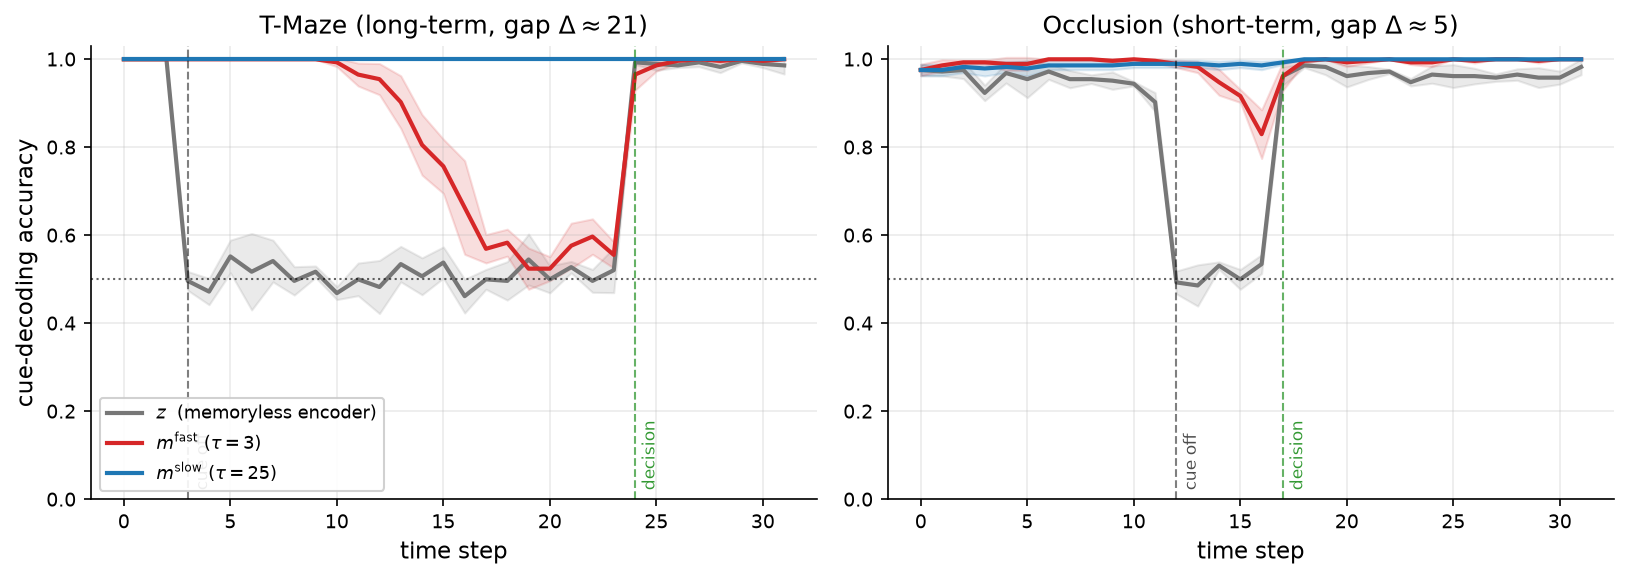
\includegraphics[width=0.82\linewidth]{figures/fig_dissociation.png}
\caption*{\textbf{Figure 1.} Cue-decoding accuracy over time (mean\(\pm\)std, 3 seeds), design `both`. Left: T-Maze (long). Right: Occlusion (short). Dotted = chance; black/green dashed = cue-off / decision.}
\end{figure}

Table 1 reports availability at the decision step:

\textbf{Table 1 --- Availability at the decision (design
\texttt{both}, 3 seeds).} Cue decodable from each stream.

{\def\LTcaptype{none} % do not increment counter
\begin{longtable}[]{@{}
  >{\raggedright\arraybackslash}p{(\linewidth - 8\tabcolsep) * \real{0.1579}}
  >{\raggedleft\arraybackslash}p{(\linewidth - 8\tabcolsep) * \real{0.2105}}
  >{\raggedleft\arraybackslash}p{(\linewidth - 8\tabcolsep) * \real{0.2105}}
  >{\raggedleft\arraybackslash}p{(\linewidth - 8\tabcolsep) * \real{0.2105}}
  >{\raggedleft\arraybackslash}p{(\linewidth - 8\tabcolsep) * \real{0.2105}}@{}}
\toprule\noalign{}
\begin{minipage}[b]{\linewidth}\raggedright
env
\end{minipage} & \begin{minipage}[b]{\linewidth}\raggedleft
gap \(\Delta\)
\end{minipage} & \begin{minipage}[b]{\linewidth}\raggedleft
\(z\) (memoryless)
\end{minipage} & \begin{minipage}[b]{\linewidth}\raggedleft
\(m^{\text{fast}}\) (\(\tau{=}3\))
\end{minipage} & \begin{minipage}[b]{\linewidth}\raggedleft
\(m^{\text{slow}}\) (\(\tau{=}25\))
\end{minipage} \\
\midrule\noalign{}
\endhead
\bottomrule\noalign{}
\endlastfoot
Occlusion & 5 & 0.46 & \textbf{0.90} & 0.99 \\
Recall & 15 & 0.33 & 0.33 & \textbf{0.55} \\
T-Maze & 21 & 0.53 & 0.49 & \textbf{1.00} \\
Distractor & 23 & 0.54 & 0.52 & \textbf{1.00} \\
\end{longtable}
}

\subsection{The matched timescale drives the decision
(usage)}\label{the-matched-timescale-drives-the-decision-usage}

\textbf{Table 2 --- Usage: cue decodable from the model's
prediction (matched probe, 5 seeds, mean\(\pm\)std).} Higher is
better; chance in last column.

{\def\LTcaptype{none} % do not increment counter
\begin{longtable}[]{@{}
  >{\raggedright\arraybackslash}p{(\linewidth - 12\tabcolsep) * \real{0.1111}}
  >{\raggedleft\arraybackslash}p{(\linewidth - 12\tabcolsep) * \real{0.1481}}
  >{\raggedleft\arraybackslash}p{(\linewidth - 12\tabcolsep) * \real{0.1481}}
  >{\raggedleft\arraybackslash}p{(\linewidth - 12\tabcolsep) * \real{0.1481}}
  >{\raggedleft\arraybackslash}p{(\linewidth - 12\tabcolsep) * \real{0.1481}}
  >{\raggedleft\arraybackslash}p{(\linewidth - 12\tabcolsep) * \real{0.1481}}
  >{\raggedleft\arraybackslash}p{(\linewidth - 12\tabcolsep) * \real{0.1481}}@{}}
\toprule\noalign{}
\begin{minipage}[b]{\linewidth}\raggedright
env
\end{minipage} & \begin{minipage}[b]{\linewidth}\raggedleft
gap \(\Delta\)
\end{minipage} & \begin{minipage}[b]{\linewidth}\raggedleft
none (vanilla)
\end{minipage} & \begin{minipage}[b]{\linewidth}\raggedleft
short
\end{minipage} & \begin{minipage}[b]{\linewidth}\raggedleft
long
\end{minipage} & \begin{minipage}[b]{\linewidth}\raggedleft
both
\end{minipage} & \begin{minipage}[b]{\linewidth}\raggedleft
chance
\end{minipage} \\
\midrule\noalign{}
\endhead
\bottomrule\noalign{}
\endlastfoot
T-Maze & 21 & 0.50 \(\pm\).02 & 0.50 \(\pm\).03 &
\textbf{0.85 \(\pm\).09} & 0.84 \(\pm\).07 & 0.50 \\
Distractor & 23 & 0.55 \(\pm\).03 & 0.54 \(\pm\).03 &
\textbf{0.88 \(\pm\).09} & 0.85 \(\pm\).07 & 0.50 \\
Recall & 15 & 0.37 \(\pm\).03 & 0.39 \(\pm\).05 & 0.45
\(\pm\).07 & \textbf{0.45 \(\pm\).04} & 0.33 \\
Occlusion & 5 & 0.51 \(\pm\).04 & 0.54 \(\pm\).05 &
\textbf{0.59 \(\pm\).04} & 0.57 \(\pm\).06 & 0.50 \\
\end{longtable}
}

On the long-horizon tasks the \texttt{long}/\texttt{both} designs lift
decision-usage well above the vanilla baseline and chance with low
variance; \texttt{none}/\texttt{short} stay at chance (Figure 2).

\begin{figure}[t]
\centering
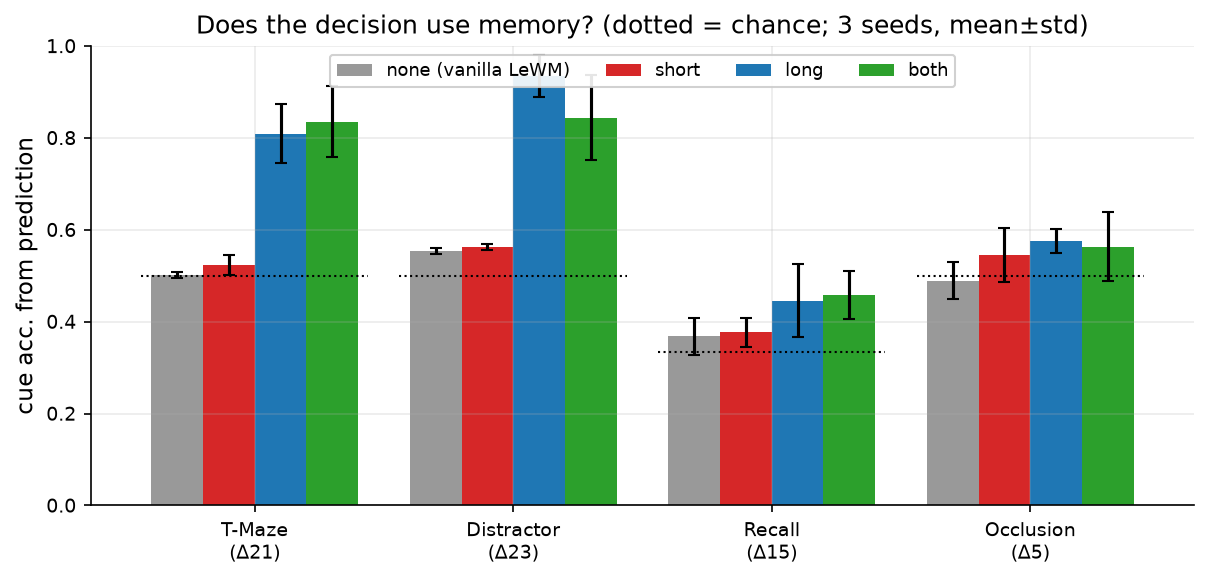
\includegraphics[width=0.82\linewidth]{figures/fig_usage_bar.png}
\caption*{\textbf{Figure 2.} Cue decodable from the model's prediction across envs and designs (3 seeds, mean\(\pm\)std; dotted = chance).}
\end{figure}

\subsection{Memory extends the usable horizon; the finite window
cliffs}\label{memory-extends-the-usable-horizon-the-finite-window-cliffs}

Sweeping the cue\(\to\)decision gap \(\Delta\) on T-Maze (Table
3, Figure 3) shows the vanilla baseline flat at chance for every
\(\Delta\) beyond its 3-frame window, while the memory model holds
high usage and \textbf{degrades gracefully}, approaching chance only as
\(\Delta\to\tau_{\text{slow}}\).

\textbf{Table 3 --- T-Maze gap sweep: usage vs.~gap
\(\Delta\) (window \(h{=}3\), \(\tau_{\text{slow}}{=}25\); 3 seeds, mean).}

{\def\LTcaptype{none} % do not increment counter
\begin{longtable}[]{@{}
  >{\raggedright\arraybackslash}p{(\linewidth - 14\tabcolsep) * \real{0.0968}}
  >{\raggedleft\arraybackslash}p{(\linewidth - 14\tabcolsep) * \real{0.1290}}
  >{\raggedleft\arraybackslash}p{(\linewidth - 14\tabcolsep) * \real{0.1290}}
  >{\raggedleft\arraybackslash}p{(\linewidth - 14\tabcolsep) * \real{0.1290}}
  >{\raggedleft\arraybackslash}p{(\linewidth - 14\tabcolsep) * \real{0.1290}}
  >{\raggedleft\arraybackslash}p{(\linewidth - 14\tabcolsep) * \real{0.1290}}
  >{\raggedleft\arraybackslash}p{(\linewidth - 14\tabcolsep) * \real{0.1290}}
  >{\raggedleft\arraybackslash}p{(\linewidth - 14\tabcolsep) * \real{0.1290}}@{}}
\toprule\noalign{}
\begin{minipage}[b]{\linewidth}\raggedright
\(\Delta\)
\end{minipage} & \begin{minipage}[b]{\linewidth}\raggedleft
3
\end{minipage} & \begin{minipage}[b]{\linewidth}\raggedleft
9
\end{minipage} & \begin{minipage}[b]{\linewidth}\raggedleft
15
\end{minipage} & \begin{minipage}[b]{\linewidth}\raggedleft
21
\end{minipage} & \begin{minipage}[b]{\linewidth}\raggedleft
27
\end{minipage} & \begin{minipage}[b]{\linewidth}\raggedleft
33
\end{minipage} & \begin{minipage}[b]{\linewidth}\raggedleft
39
\end{minipage} \\
\midrule\noalign{}
\endhead
\bottomrule\noalign{}
\endlastfoot
vanilla (none) & 0.55 & 0.55 & 0.44 & 0.53 & 0.44 & 0.48 & 0.45 \\
memory (both) & \textbf{0.98} & \textbf{0.94} & \textbf{0.88} &
\textbf{0.87} & \textbf{0.83} & \textbf{0.77} & \textbf{0.64} \\
\end{longtable}
}

\begin{figure}[t]
\centering
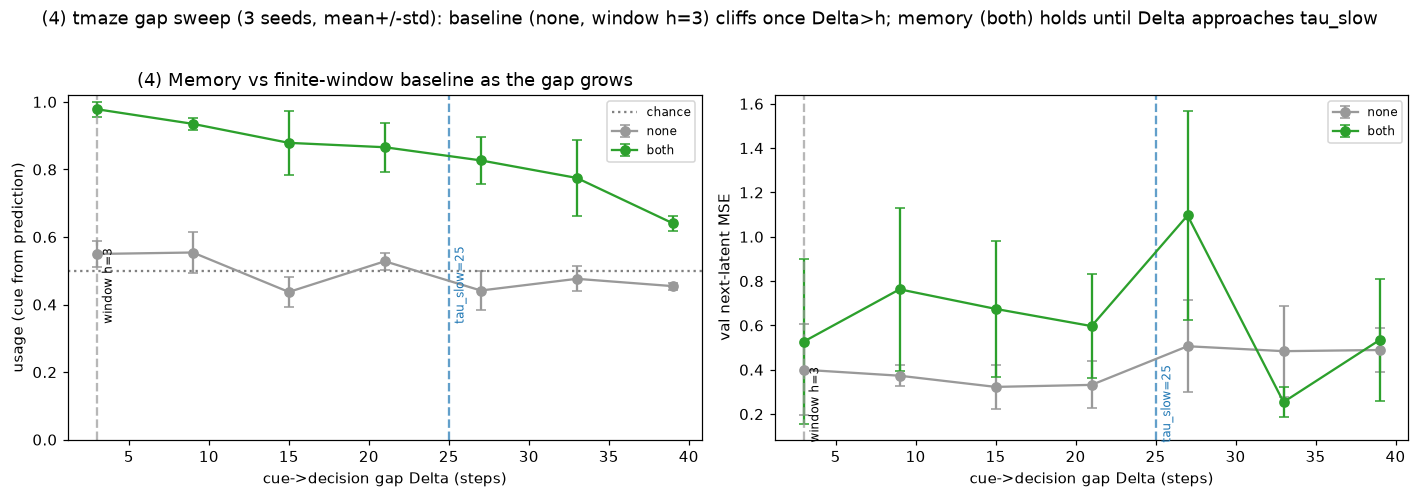
\includegraphics[width=0.82\linewidth]{figures/exp4_gap_sweep.png}
\caption*{\textbf{Figure 3.} Memory vs. finite-window baseline as the gap grows. Left: usage. Right: MSE (noisy; see \S{}5.4).}
\end{figure}

Sweeping the slow-bank horizon \(\tau_{\text{slow}}\) at fixed gap \(\Delta{=}21\)
(Table 4) confirms the duration is the operative knob: a too-short slow
bank (\(\tau{=}3\)) cannot hold the cue at all (availability at
chance), and once \(\tau_{\text{slow}}\gtrsim\Delta\) the decision recovers it.

\textbf{Table 4 --- T-Maze \(\tau_{\text{slow}}\) sweep (\(\Delta{=}21\),
design \texttt{both}; 3 seeds, mean).}

{\def\LTcaptype{none} % do not increment counter
\begin{longtable}[]{@{}
  >{\raggedright\arraybackslash}p{(\linewidth - 12\tabcolsep) * \real{0.1111}}
  >{\raggedleft\arraybackslash}p{(\linewidth - 12\tabcolsep) * \real{0.1481}}
  >{\raggedleft\arraybackslash}p{(\linewidth - 12\tabcolsep) * \real{0.1481}}
  >{\raggedleft\arraybackslash}p{(\linewidth - 12\tabcolsep) * \real{0.1481}}
  >{\raggedleft\arraybackslash}p{(\linewidth - 12\tabcolsep) * \real{0.1481}}
  >{\raggedleft\arraybackslash}p{(\linewidth - 12\tabcolsep) * \real{0.1481}}
  >{\raggedleft\arraybackslash}p{(\linewidth - 12\tabcolsep) * \real{0.1481}}@{}}
\toprule\noalign{}
\begin{minipage}[b]{\linewidth}\raggedright
\(\tau_{\text{slow}}\)
\end{minipage} & \begin{minipage}[b]{\linewidth}\raggedleft
3
\end{minipage} & \begin{minipage}[b]{\linewidth}\raggedleft
6
\end{minipage} & \begin{minipage}[b]{\linewidth}\raggedleft
12
\end{minipage} & \begin{minipage}[b]{\linewidth}\raggedleft
21
\end{minipage} & \begin{minipage}[b]{\linewidth}\raggedleft
30
\end{minipage} & \begin{minipage}[b]{\linewidth}\raggedleft
45
\end{minipage} \\
\midrule\noalign{}
\endhead
\bottomrule\noalign{}
\endlastfoot
availability (\(m^{\text{slow}}\)) & 0.47 & 0.99 & 1.00 & 1.00 & 1.00 &
1.00 \\
usage & 0.50 & 0.54 & 0.66 & 0.89 & 0.78 & 0.94 \\
\end{longtable}
}

\subsection{\texorpdfstring{What does \emph{not} hold up: raw MSE and
learned
decay}{What does not hold up: raw MSE and learned decay}}\label{what-does-not-hold-up-raw-mse-and-learned-decay}

\textbf{Prediction MSE is a decoupled instrument.} Memory lowers MSE on
some envs (Occlusion \texttt{none} \(0.46\!\to\!\) \texttt{both}
\(0.25\pm.03\)) but is noisy elsewhere and even \emph{raises} it where
stochastic distractors dominate the loss; in the \(\tau_{\text{slow}}\) sweep,
\(\tau{=}3\) has the \emph{lowest} MSE yet chance usage. The cue is a
small sub-space of the global latent, so MSE does not track memory
quality --- the probes do.

\textbf{Table 5 --- Validation next-latent MSE (3 seeds,
mean\(\pm\)std). Lower is better.}

{\def\LTcaptype{none} % do not increment counter
\begin{longtable}[]{@{}
  >{\raggedright\arraybackslash}p{(\linewidth - 8\tabcolsep) * \real{0.1579}}
  >{\raggedleft\arraybackslash}p{(\linewidth - 8\tabcolsep) * \real{0.2105}}
  >{\raggedleft\arraybackslash}p{(\linewidth - 8\tabcolsep) * \real{0.2105}}
  >{\raggedleft\arraybackslash}p{(\linewidth - 8\tabcolsep) * \real{0.2105}}
  >{\raggedleft\arraybackslash}p{(\linewidth - 8\tabcolsep) * \real{0.2105}}@{}}
\toprule\noalign{}
\begin{minipage}[b]{\linewidth}\raggedright
env
\end{minipage} & \begin{minipage}[b]{\linewidth}\raggedleft
none
\end{minipage} & \begin{minipage}[b]{\linewidth}\raggedleft
short
\end{minipage} & \begin{minipage}[b]{\linewidth}\raggedleft
long
\end{minipage} & \begin{minipage}[b]{\linewidth}\raggedleft
both
\end{minipage} \\
\midrule\noalign{}
\endhead
\bottomrule\noalign{}
\endlastfoot
T-Maze & 0.76 \(\pm\).44 & 0.47 \(\pm\).17 & 0.62
\(\pm\).53 & 0.55 \(\pm\).32 \\
Occlusion & 0.46 \(\pm\).18 & 0.54 \(\pm\).36 & 0.39
\(\pm\).12 & \textbf{0.25 \(\pm\).03} \\
Recall & 0.76 \(\pm\).46 & \textbf{0.33 \(\pm\).11} & 0.56
\(\pm\).37 & 0.73 \(\pm\).49 \\
Distractor & \textbf{0.39 \(\pm\).12} & 0.41 \(\pm\).16 &
0.57 \(\pm\).19 & 0.52 \(\pm\).21 \\
TwoRoom (control) & \textbf{0.48} & --- & --- &
0.48 \\
\end{longtable}
}

\textbf{Learned decay does not self-tune.} Making \(\alpha\)
learnable leaves the horizons near their initialization for every
environment --- across 3 seeds the learned \(\tau_{\text{slow}}\) is
\(23.9\text{–}24.4\) regardless of the task gap (5 / 15 / 21 / 23), with std
\(\le0.4\) --- i.e., it does \emph{not} track the gap; the
gradient signal on a scalar decay is weak. The practical lever is
therefore \emph{choosing} timescales, which is precisely why two banks
spanning a \emph{range} of horizons is the right design.

\subsection{Control}\label{control}

On the fully-observable \textbf{TwoRoom}, \texttt{none} and
\texttt{both} are indistinguishable on the held-out set (Table 5),
confirming the gains above are memory-specific rather than added
capacity.

\subsection{Standard benchmark: POPGym Arcade (5 tasks \(\times\) 5
seeds)}\label{standard-benchmark-popgym-arcade-5-tasks-xxmath00149xx-5-seeds}

We evaluate on \textbf{five} memory-centric POMDPs from \textbf{POPGym
Arcade} {[}Morad et al.{]} --- CountRecall, AutoEncode,
BattleShip, MineSweeper, Navigator --- pixel observations,
discrete actions (one-hot). These have no clean cue label, so we report
next-latent val MSE and memory-ablation influence (\textbf{5 seeds};
\texttt{lewm-memory-popgym}), comparing vanilla \texttt{none} to the
fixed K-bank \texttt{multi} (our best design, \S{}5.11).

\textbf{Table 6 --- POPGym Arcade: next-latent val MSE
(lower=better) and K-bank influence (5 seeds, mean).}

{\def\LTcaptype{none} % do not increment counter
\begin{longtable}[]{@{}lrrrr@{}}
\toprule\noalign{}
task & none (vanilla) & multi (K-bank) & reduction & \(\mathcal I_{\text{slow}}\) \\
\midrule\noalign{}
\endhead
\bottomrule\noalign{}
\endlastfoot
CountRecall & 1.08 & \textbf{0.51} & \(-\)53\% & 10.0 \\
BattleShip & 0.80 & \textbf{0.26} & \(-\)68\% & 12.5 \\
Navigator & 0.61 & \textbf{0.48} & \(-\)21\% & 14.6 \\
AutoEncode & 0.65 & \textbf{0.55} & \(-\)15\% & 5.9 \\
MineSweeper & 0.020 & 0.019 & \(-\)2\% & 0.2 \\
\end{longtable}
}

\begin{figure}[t]
\centering
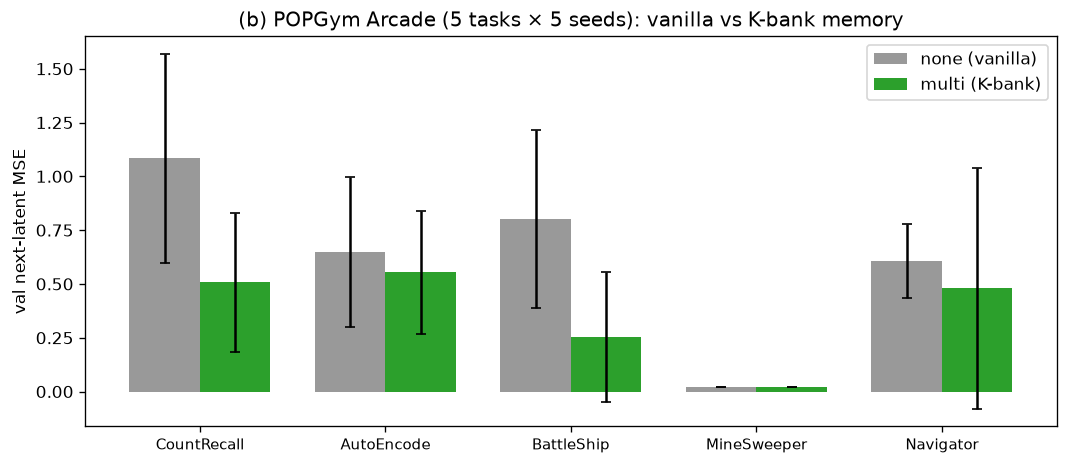
\includegraphics[width=0.82\linewidth]{figures/fig_popgym_broad.png}
\caption*{\textbf{Figure 4.} POPGym Arcade, 5 tasks \(\times\) 5 seeds: vanilla LeWM vs the fixed K-bank memory (next-latent val MSE).}
\end{figure}

The K-bank memory reduces prediction error on the four memory-demanding
tasks (\textbf{\(-\)15\% to \(-\)68\%}) with large
memory influence (\(\mathcal I\approx6\text{–}15\)), and leaves the near-trivial
MineSweeper (val \(\approx\)0.02; almost nothing to predict,
\(\mathcal I\approx0\)) unchanged --- memory helps where it is needed
and is inert where it is not. So the primitive transfers to a standard
benchmark at the \(\ge\)5-task\(\times\)5-seed bar.

\subsection{\texorpdfstring{Counterfactual memory swap: the memory
\emph{causally} drives the
prediction}{Counterfactual memory swap: the memory causally drives the prediction}}\label{counterfactual-memory-swap-the-memory-causally-drives-the-prediction}

Probes show information is decodable, but not that the predictor
\emph{uses} it. We therefore intervene: for each episode \emph{i} we
predict the reveal-latent using \emph{i}'s current frames and actions
but \textbf{another episode \emph{j}'s memory banks} (with
cue{[}\emph{j}{]}\(\ne\)cue{[}\emph{i}{]}), and apply a matched
probe.

\textbf{Table 7 --- Counterfactual memory swap (design
\texttt{both}, 3 seeds, mean\(\pm\)std).} Does the prediction
follow the \emph{injected} memory or the \emph{current} frame?

{\def\LTcaptype{none} % do not increment counter
\begin{longtable}[]{@{}
  >{\raggedright\arraybackslash}p{(\linewidth - 8\tabcolsep) * \real{0.1579}}
  >{\raggedleft\arraybackslash}p{(\linewidth - 8\tabcolsep) * \real{0.2105}}
  >{\raggedleft\arraybackslash}p{(\linewidth - 8\tabcolsep) * \real{0.2105}}
  >{\raggedleft\arraybackslash}p{(\linewidth - 8\tabcolsep) * \real{0.2105}}
  >{\raggedleft\arraybackslash}p{(\linewidth - 8\tabcolsep) * \real{0.2105}}@{}}
\toprule\noalign{}
\begin{minipage}[b]{\linewidth}\raggedright
env
\end{minipage} & \begin{minipage}[b]{\linewidth}\raggedleft
own memory \(\to\) cue (control)
\end{minipage} & \begin{minipage}[b]{\linewidth}\raggedleft
\textbf{swapped memory \(\to\) swapped cue}
\end{minipage} & \begin{minipage}[b]{\linewidth}\raggedleft
swapped \(\to\) current-frame cue
\end{minipage} & \begin{minipage}[b]{\linewidth}\raggedleft
chance
\end{minipage} \\
\midrule\noalign{}
\endhead
\bottomrule\noalign{}
\endlastfoot
T-Maze & 0.85 & \textbf{0.83} & 0.17 & 0.50 \\
Distractor & 0.87 & \textbf{0.79} & 0.21 & 0.50 \\
Recall & 0.41 & 0.40 & 0.25 & 0.33 \\
Occlusion & 0.58 & 0.58 & 0.43 & 0.50 \\
\end{longtable}
}

\begin{figure}[t]
\centering
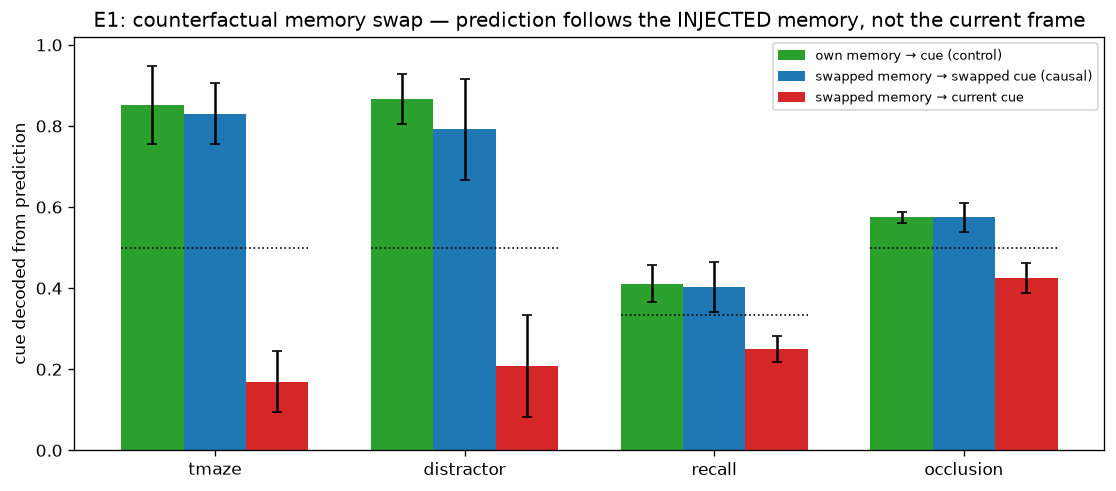
\includegraphics[width=0.82\linewidth]{figures/fig_causal_swap.png}
\caption*{\textbf{Figure 5.} Swapping the memory bank between episodes with different cues. On long-gap tasks the prediction tracks the \textbf{injected} cue (follow-memory \(\approx\) follow-self), while the current-frame cue collapses to ~chance.}
\end{figure}

On the long-gap tasks, swapping the memory bank \textbf{flips the
prediction to the injected cue} (follow-memory \(\approx\) the
own-memory control) while reading the current frame collapses to
\textasciitilde chance --- direct causal evidence that the EMA
banks control the prediction, not merely carry decodable information.
This is the decisive test that probe decodability alone cannot provide.

\subsection{Mechanistic attribution: which frames each step
reads}\label{mechanistic-attribution-which-frames-each-step-reads}

To open the box further we attribute each step's next-latent prediction
(i) to its memory banks and (ii) to source frames. \textbf{Per-step bank
influence} \(I_c(t)=\lVert \hat y_t-\hat y_t(\text{ablate }c)\rVert\) reveals the dissociation at the mechanism
level: on \textbf{T-Maze (long gap)} the \emph{slow} bank dominates the
prediction at \emph{every} step (\(I_{\text{slow}}\approx2.15>I_{\text{fast}}\approx1.8\)), whereas on
\textbf{Occlusion (short gap)} the \emph{fast} bank dominates
(\(I_{\text{fast}}\approx2.18>I_{\text{slow}}\approx2.07\)). \textbf{Frame attribution} \(\lVert\partial\hat y_{\text{rev}}/\partial z_s\rVert\) at the
decision step is dominated by the recent \(h\)-frame window (the
direct path), but the \emph{slow} exponential kernel is the only pathway
that reaches the early cue frames --- and the decision shows a
real attribution bump there --- confirming that the
long-horizon decision reads the early cue \emph{through the slow bank}.

\begin{figure}[t]
\centering
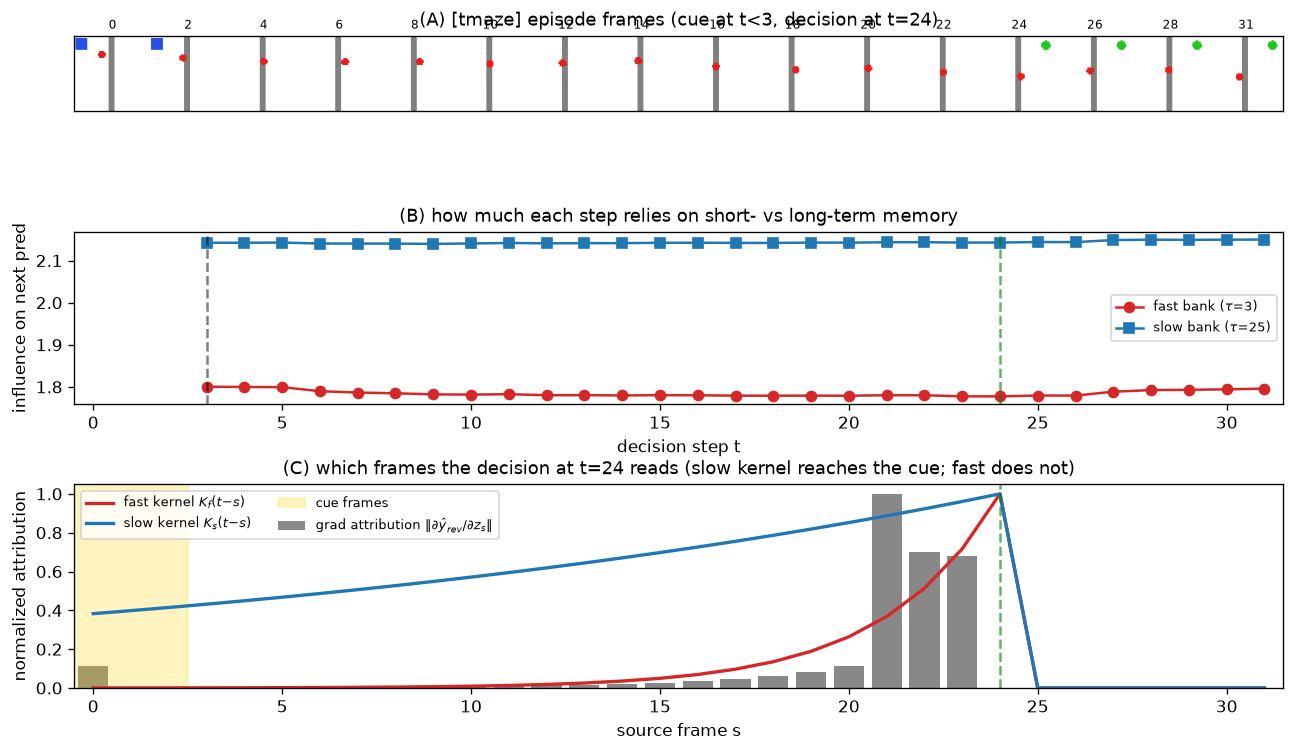
\includegraphics[width=0.47\linewidth]{figures/fig_attribution_tmaze.png}\hfill
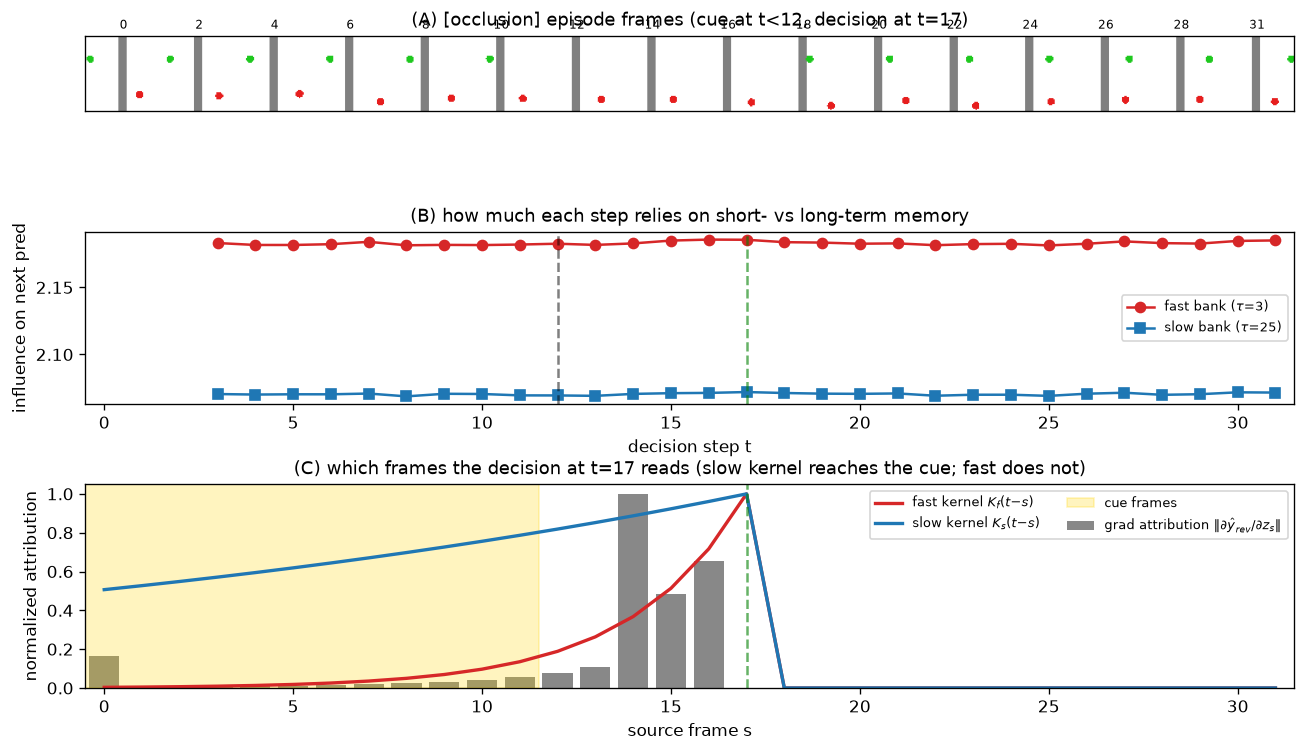
\includegraphics[width=0.47\linewidth]{figures/fig_attribution_occlusion.png}
\caption*{\textbf{Figures 6--7.} Memory-attribution timeline. (A) episode frames; (B) per-step fast vs slow bank influence on the next prediction; (C) gradient attribution of the decision over source frames, with the fast/slow kernels overlaid and cue frames shaded. T-Maze: slow bank dominates and reaches the cue; Occlusion: fast bank dominates.}
\end{figure}

\subsection{Partially-observable variants of the paper's own
tasks}\label{partially-observable-variants-of-the-papers-own-tasks}

To test the effect on the \emph{paper's task semantics} (not just our
toy suite), we build PO variants of LeWorldModel's four benchmark envs
--- Two-Room, Reacher, Push-T, OGBench-Cube --- as
lightweight pixel proxies where the goal is shown briefly then hidden
(so it must be remembered; \texttt{lewm-memory-paperpo}, 3 seeds,
4-class cue, chance 0.25).

\textbf{Table 8 --- Paper-task PO variants: usage (cue
decodable from the prediction, 3 seeds, mean\(\pm\)std).}

{\def\LTcaptype{none} % do not increment counter
\begin{longtable}[]{@{}
  >{\raggedright\arraybackslash}p{(\linewidth - 12\tabcolsep) * \real{0.1111}}
  >{\raggedleft\arraybackslash}p{(\linewidth - 12\tabcolsep) * \real{0.1481}}
  >{\raggedleft\arraybackslash}p{(\linewidth - 12\tabcolsep) * \real{0.1481}}
  >{\raggedleft\arraybackslash}p{(\linewidth - 12\tabcolsep) * \real{0.1481}}
  >{\raggedleft\arraybackslash}p{(\linewidth - 12\tabcolsep) * \real{0.1481}}
  >{\raggedleft\arraybackslash}p{(\linewidth - 12\tabcolsep) * \real{0.1481}}
  >{\raggedleft\arraybackslash}p{(\linewidth - 12\tabcolsep) * \real{0.1481}}@{}}
\toprule\noalign{}
\begin{minipage}[b]{\linewidth}\raggedright
env (paper task)
\end{minipage} & \begin{minipage}[b]{\linewidth}\raggedleft
gap \(\Delta\)
\end{minipage} & \begin{minipage}[b]{\linewidth}\raggedleft
none (vanilla)
\end{minipage} & \begin{minipage}[b]{\linewidth}\raggedleft
short
\end{minipage} & \begin{minipage}[b]{\linewidth}\raggedleft
long
\end{minipage} & \begin{minipage}[b]{\linewidth}\raggedleft
both
\end{minipage} & \begin{minipage}[b]{\linewidth}\raggedleft
chance
\end{minipage} \\
\midrule\noalign{}
\endhead
\bottomrule\noalign{}
\endlastfoot
Two-Room-PO & 19 & 0.23 \(\pm\).05 & 0.25 \(\pm\).01 &
\textbf{0.40 \(\pm\).03} & 0.38 \(\pm\).05 & 0.25 \\
Push-T-PO & 17 & 0.31 \(\pm\).04 & 0.32 \(\pm\).02 &
\textbf{0.48 \(\pm\).06} & \textbf{0.48 \(\pm\).04} &
0.25 \\
OGBench-Cube-PO & 15 & 0.26 \(\pm\).00 & 0.31 \(\pm\).02 &
\textbf{0.42 \(\pm\).03} & 0.38 \(\pm\).04 & 0.25 \\
Reacher-PO & 13 & 0.24 \(\pm\).02 & 0.26 \(\pm\).02 &
\textbf{0.38 \(\pm\).01} & 0.36 \(\pm\).05 & 0.25 \\
\end{longtable}
}

Across all four, \texttt{long}/\texttt{both} lift decision-usage above
chance while \texttt{none}/\texttt{short} stay at chance; availability
(design \texttt{both}) is \texttt{z}\(\approx\)0.25,
\texttt{m\^{}\{fast\}}\(\approx\)0.25 (gaps 13--19 exceed
\(\tau_{\text{fast}}{=}3\)), \texttt{m\^{}\{slow\}}=1.00 --- only the slow
bank carries the goal cue. So the short/long dissociation holds on PO
versions of the paper's \emph{own} tasks, not only our custom suite.
\emph{Caveat:} these are lightweight pixel proxies (not the original
MuJoCo/pymunk/OGBench simulators), and with continuous joint-angle
actions for Reacher; the effect is moderate (4-class) but consistent.

\subsection{Downstream closed-loop
control}\label{downstream-closed-loop-control}

Finally we close the loop: an interactive memory T-Maze where the agent
must \emph{navigate} to the arm indicated by a cue shown briefly and
then hidden (\texttt{lewm/envs/control\_envs.py}). The agent gathers a
short context by moving toward the junction, the world model
\textbf{imagines the goal} by rolling its latent forward to the reveal
step (memory-aware rollout), and a linear read-out of that imagined
latent picks the arm. Success = committing to the cued arm.

\textbf{Table 9 --- Closed-loop T-Maze control success (3
seeds, mean\(\pm\)std).}

{\def\LTcaptype{none} % do not increment counter
\begin{longtable}[]{@{}
  >{\raggedright\arraybackslash}p{(\linewidth - 6\tabcolsep) * \real{0.2000}}
  >{\raggedleft\arraybackslash}p{(\linewidth - 6\tabcolsep) * \real{0.2667}}
  >{\raggedleft\arraybackslash}p{(\linewidth - 6\tabcolsep) * \real{0.2667}}
  >{\raggedleft\arraybackslash}p{(\linewidth - 6\tabcolsep) * \real{0.2667}}@{}}
\toprule\noalign{}
\begin{minipage}[b]{\linewidth}\raggedright
design
\end{minipage} & \begin{minipage}[b]{\linewidth}\raggedleft
success
\end{minipage} & \begin{minipage}[b]{\linewidth}\raggedleft
memory ablated at test
\end{minipage} & \begin{minipage}[b]{\linewidth}\raggedleft
chance
\end{minipage} \\
\midrule\noalign{}
\endhead
\bottomrule\noalign{}
\endlastfoot
none (vanilla) & 0.48 \(\pm\).00 & 0.48 \(\pm\).00 & 0.50 \\
short & \textbf{1.00 \(\pm\).00} & 0.48 \(\pm\).00 & 0.50 \\
long & \textbf{1.00 \(\pm\).00} & 0.49 \(\pm\).02 & 0.50 \\
both & \textbf{1.00 \(\pm\).00} & 0.51 \(\pm\).02 & 0.50 \\
\end{longtable}
}

\begin{figure}[t]
\centering
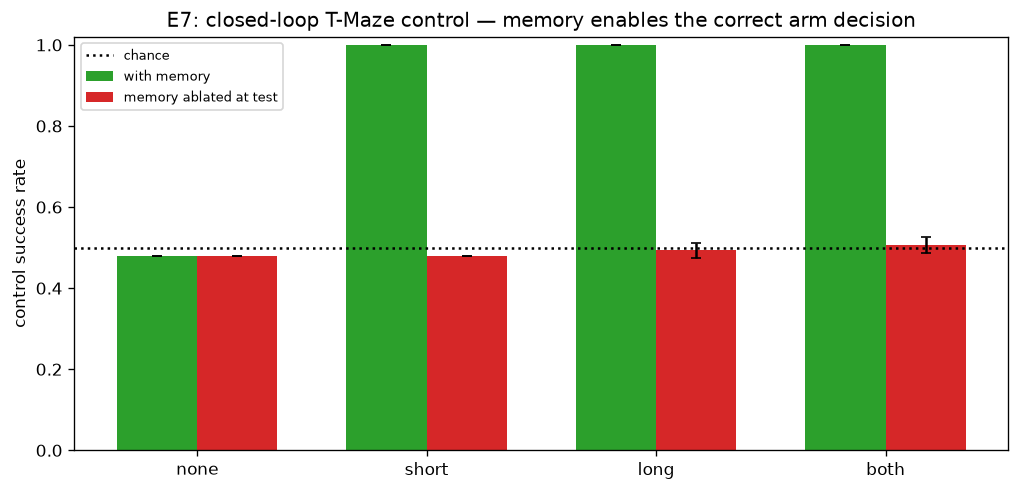
\includegraphics[width=0.82\linewidth]{figures/fig_E7_planning.png}
\caption*{\textbf{Figure 8.} Closed-loop control. Memory designs reach the cued arm reliably (1.00) while vanilla LeWM is at chance; ablating the memory \textbf{at test time} collapses every memory design to chance.}
\end{figure}

Memory \textbf{causally enables the downstream decision}: with memory
the agent reaches the correct arm every time, vanilla LeWM cannot, and
removing the memory at test time breaks it (\(\to\) chance). This
is the decisive control-level analogue of \S{}5.7. \emph{Honest
note:} \texttt{short} also succeeds at this cue\(\to\)decision gap
because the linear read-out exploits even residual fast-bank signal (the
availability-vs-readout effect of \S{}5.4); the clean causal
contrast here is memory-vs-none and the test-time ablation, not
short-vs-long.

\subsection{Is two-timescale EMA the right primitive?
(baselines)}\label{is-two-timescale-ema-the-right-primitive-baselines}

We compare the fixed-EMA designs against three \emph{learned} memories
--- a \textbf{log-spaced fixed K-bank} (\texttt{multi},
\(\tau\in\{2,4,8,16,32,64\}\), no tuning), a \textbf{learned GRU}, a \textbf{learned
diagonal-SSM / RetNet-lite} (\texttt{ssm}, per-channel learned decay),
and an \textbf{episodic-retrieval} bank (\texttt{retrieval}, causal
attention over stored latents) --- and a \textbf{long-context
predictor} (window \(h\)). Usage (cue from prediction):

\textbf{Table 10 --- Memory-mechanism comparison (usage;
fixed-EMA 5 seeds, learned 3 seeds, mean\(\pm\)std).}

{\def\LTcaptype{none} % do not increment counter
\begin{longtable}[]{@{}
  >{\raggedright\arraybackslash}p{(\linewidth - 14\tabcolsep) * \real{0.0968}}
  >{\raggedleft\arraybackslash}p{(\linewidth - 14\tabcolsep) * \real{0.1290}}
  >{\raggedleft\arraybackslash}p{(\linewidth - 14\tabcolsep) * \real{0.1290}}
  >{\raggedleft\arraybackslash}p{(\linewidth - 14\tabcolsep) * \real{0.1290}}
  >{\raggedleft\arraybackslash}p{(\linewidth - 14\tabcolsep) * \real{0.1290}}
  >{\raggedleft\arraybackslash}p{(\linewidth - 14\tabcolsep) * \real{0.1290}}
  >{\raggedleft\arraybackslash}p{(\linewidth - 14\tabcolsep) * \real{0.1290}}
  >{\raggedleft\arraybackslash}p{(\linewidth - 14\tabcolsep) * \real{0.1290}}@{}}
\toprule\noalign{}
\begin{minipage}[b]{\linewidth}\raggedright
env
\end{minipage} & \begin{minipage}[b]{\linewidth}\raggedleft
none
\end{minipage} & \begin{minipage}[b]{\linewidth}\raggedleft
long
\end{minipage} & \begin{minipage}[b]{\linewidth}\raggedleft
both
\end{minipage} & \begin{minipage}[b]{\linewidth}\raggedleft
\textbf{multi (fixed)}
\end{minipage} & \begin{minipage}[b]{\linewidth}\raggedleft
gru
\end{minipage} & \begin{minipage}[b]{\linewidth}\raggedleft
ssm
\end{minipage} & \begin{minipage}[b]{\linewidth}\raggedleft
retrieval
\end{minipage} \\
\midrule\noalign{}
\endhead
\bottomrule\noalign{}
\endlastfoot
T-Maze & 0.50 \(\pm\).02 & 0.85 \(\pm\).09 & 0.84
\(\pm\).07 & \textbf{0.99 \(\pm\).01} & 0.54
\(\pm\).05 & 0.58 \(\pm\).07 & 0.72 \(\pm\).16 \\
Distractor & 0.55 \(\pm\).03 & 0.88 \(\pm\).09 & 0.85
\(\pm\).07 & \textbf{0.99 \(\pm\).01} & 0.59
\(\pm\).02 & 0.56 \(\pm\).04 & 0.68 \(\pm\).12 \\
Recall & 0.37 \(\pm\).03 & 0.45 \(\pm\).07 & 0.45
\(\pm\).04 & \textbf{0.47 \(\pm\).01} & 0.45
\(\pm\).02 & 0.46 \(\pm\).03 & 0.52 \(\pm\).01 \\
Occlusion & 0.51 \(\pm\).04 & 0.59 \(\pm\).04 & 0.57
\(\pm\).06 & \textbf{0.81 \(\pm\).06} & 0.68
\(\pm\).18 & 0.58 \(\pm\).04 & 0.61 \(\pm\).05 \\
\end{longtable}
}

\textbf{Long-context predictor (T-Maze, design \texttt{none}, window
\(h\); vs EMA at \(h{=}3\)):} \(h{=}9{:}\,0.46\), \(h{=}18{:}\,0.50\),
\(h{=}21{:}\,0.50\), \(h{=}24{:}\,\mathbf{1.00}\) --- vs EMA \texttt{both}
\(0.84\) / \texttt{multi} \(0.99\) at \(h{=}3\).

Three takeaways. \textbf{(i) The fixed log-spaced K-bank is the best
design everywhere, with \emph{no} per-task \(\tau\) tuning}
--- fixing the ``learned \(\alpha\) doesn't self-tune''
weakness (\S{}5.4): \emph{spanning} horizons beats picking one.
\textbf{(ii) Every \emph{learned} memory --- GRU,
diagonal-SSM/RetNet-lite, and episodic retrieval ---
underperforms the fixed EMA on long-gap tasks} (T-Maze: gru 0.54, ssm
0.58, retrieval 0.72, all \(\ll\) multi 0.99). So it is \emph{not}
merely ``memory helps''; the \textbf{fixed exponential structure is the
right inductive bias} (no long-range credit assignment needed) in this
low-data/short-training regime. \emph{(Caveat: tuned, longer-trained
SSMs could close the gap; reported under matched budget/training.)}
\textbf{(iii) Enlarging the predictor window does not help until it
spans the whole gap} (\(h{\le}21\) stay at chance; \(h{=}24\)
reaches the cue \(\to\) 1.00, at \(O(\Delta)\) context cost)
--- whereas the EMA reaches 0.84--0.99 with
\(h{=}3\) and \(O(1)\) memory. (h=18/24 single-seed; trend
clear.)

\subsection{The horizon law,
quantified}\label{the-horizon-law-quantified}

Sweeping gap \(\Delta\) \(\times\) horizon \(\tau\) (design
\texttt{long}, T-Maze) makes the rule precise: \textbf{usage is high iff
\(\tau \gtrsim \Delta\).}

\textbf{Table 11 --- usage(\(\Delta\), \(\tau\)).}

{\def\LTcaptype{none} % do not increment counter
\begin{longtable}[]{@{}lrrr@{}}
\toprule\noalign{}
\(\Delta\) ~\(\tau\) & 4 & 16 & 64 \\
\midrule\noalign{}
\endhead
\bottomrule\noalign{}
\endlastfoot
3 & 0.92 & 1.00 & 0.98 \\
9 & 0.78 & 0.96 & 0.98 \\
21 & 0.50 & 0.89 & 0.89 \\
39 & 0.44 & 0.58 & 0.96 \\
\end{longtable}
}

\begin{figure}[t]
\centering
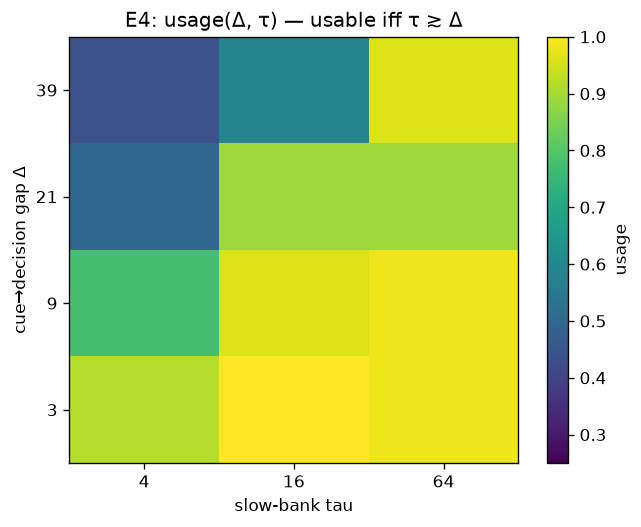
\includegraphics[width=0.47\linewidth]{figures/exp_E4_horizon_law.png}\hfill
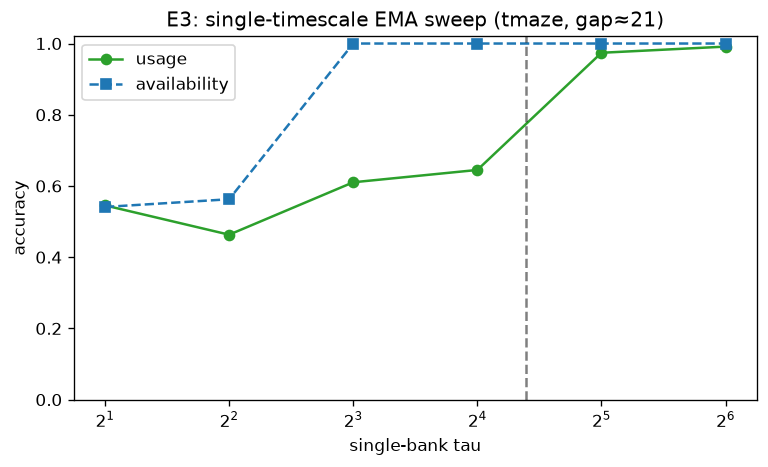
\includegraphics[width=0.47\linewidth]{figures/exp_E3_singletau.png}
\caption*{\textbf{Figures 9--10.} (9) usage(\(\Delta,\tau\)): the usable region is \(\tau\gtrsim\Delta\), matching the exponential kernel \(e^{-\Delta/\tau}\). (10) single-bank sweep at \(\Delta{\approx}21\): availability saturates by \(\tau{=}8\) but \textbf{usage keeps rising to \(\tau{=}64\)} --- quantitative confirmation that linear availability is necessary but not sufficient (\S{}5.4).}
\end{figure}

\subsection{Frozen-backbone: a drop-on for a pretrained JEPA
encoder}\label{frozen-backbone-a-drop-on-for-a-pretrained-jepa-encoder}

To show the primitive is \emph{backbone-agnostic}, we pretrain a vanilla
(memoryless) LeWM encoder, \textbf{freeze} it, and train only the memory
+ predictor on top (\texttt{-\/-freeze-encoder}; 4 envs \(\times\) 3
seeds; \texttt{lewm-memory-frozen}).

\textbf{Table 12 --- Usage with a frozen vanilla encoder (3
seeds, mean).}

{\def\LTcaptype{none} % do not increment counter
\begin{longtable}[]{@{}lrrr@{}}
\toprule\noalign{}
env & none & both & multi \\
\midrule\noalign{}
\endhead
\bottomrule\noalign{}
\endlastfoot
T-Maze & 0.49 & 0.67 & \textbf{0.84} \\
Distractor & 0.53 & 0.61 & \textbf{0.86} \\
Recall & 0.37 & 0.41 & \textbf{0.46} \\
Occlusion & 0.48 & 0.52 & \textbf{0.65} \\
\end{longtable}
}

\begin{figure}[t]
\centering
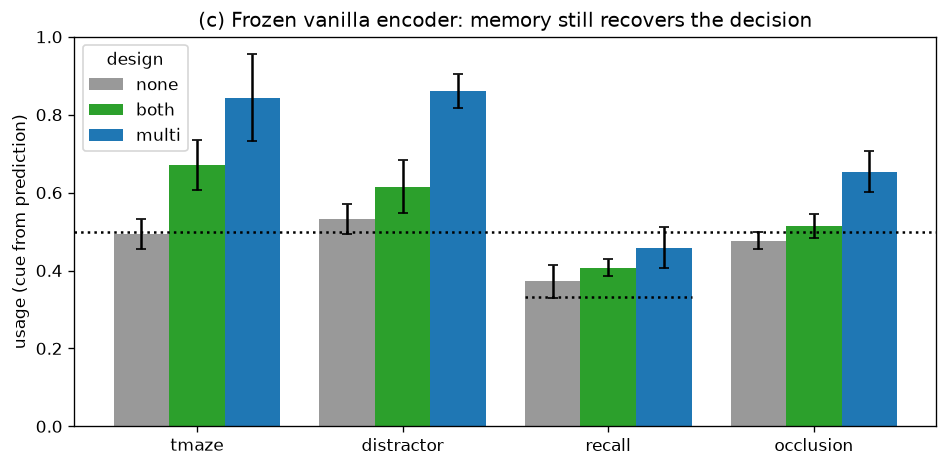
\includegraphics[width=0.82\linewidth]{figures/fig_frozen.png}
\caption*{\textbf{Figure 11.} With the encoder frozen, memory (esp. `multi`) still recovers the decision well above chance.}
\end{figure}

Even with the encoder frozen, memory recovers the decision well above
the memoryless baseline (T-Maze 0.49\(\to\)0.84, Distractor
0.53\(\to\)0.86) --- the primitive is an add-on to a
pretrained JEPA backbone, not a LeWM-specific end-to-end trick.

\textbf{A genuinely external pretrained backbone (DINO-WM-style).} The
frozen encoder above is still a \emph{vanilla LeWM} encoder. To rule out
any LeWM-specific coupling, we repeat the study with a truly external
backbone: a \textbf{frozen pretrained DINOv2 ViT-S} (21.6 M parameters,
\texttt{vit\_small\_patch14\_dinov2}, distilled on ImageNet, \emph{never
trained on these tasks} --- the DINO-WM recipe). We
interpolate the 64\(\times\)64 frames to 224, apply ImageNet
normalisation, and train only a small projector + the memory + the
predictor; the backbone stays in \texttt{eval()} throughout. We use the
matched usage probe (does the predictor's decision-point output carry
the cue?) and, as a control, the \textbf{instantaneous frozen latent}
\(z\) at the decision frame (4 envs \(\times\) \{none,
multi\} \(\times\) 2 seeds; \texttt{lewm-memory-dino}).

\textbf{Table 12b --- Frozen pretrained DINOv2 ViT-S backbone:
cue usage at the decision (2 seeds, mean).}

{\def\LTcaptype{none} % do not increment counter
\begin{longtable}[]{@{}
  >{\raggedright\arraybackslash}p{(\linewidth - 8\tabcolsep) * \real{0.1579}}
  >{\raggedleft\arraybackslash}p{(\linewidth - 8\tabcolsep) * \real{0.2105}}
  >{\raggedleft\arraybackslash}p{(\linewidth - 8\tabcolsep) * \real{0.2105}}
  >{\raggedleft\arraybackslash}p{(\linewidth - 8\tabcolsep) * \real{0.2105}}
  >{\raggedleft\arraybackslash}p{(\linewidth - 8\tabcolsep) * \real{0.2105}}@{}}
\toprule\noalign{}
\begin{minipage}[b]{\linewidth}\raggedright
env
\end{minipage} & \begin{minipage}[b]{\linewidth}\raggedleft
frozen latent \(z\)
\end{minipage} & \begin{minipage}[b]{\linewidth}\raggedleft
none (pred.)
\end{minipage} & \begin{minipage}[b]{\linewidth}\raggedleft
multi (K-bank)
\end{minipage} & \begin{minipage}[b]{\linewidth}\raggedleft
chance
\end{minipage} \\
\midrule\noalign{}
\endhead
\bottomrule\noalign{}
\endlastfoot
T-Maze (\(\Delta\)=21) & 0.57 & 0.53 & \textbf{0.86} & 0.50 \\
Distractor (\(\Delta\)=23) & 0.50 & 0.52 & \textbf{0.65} & 0.50 \\
Occlusion (\(\Delta\)=5) & 0.45 & 0.55 & 0.61 & 0.50 \\
Recall (\(\Delta\)=15, 3-way) & 0.37 & 0.38 & 0.36 & 0.33 \\
\end{longtable}
}

\begin{figure}[t]
\centering
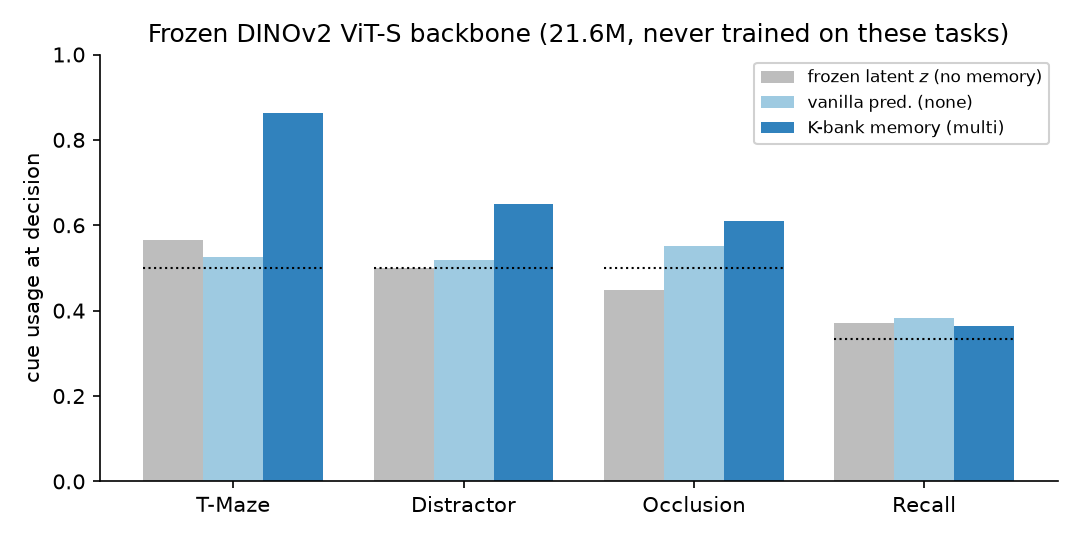
\includegraphics[width=0.82\linewidth]{figures/fig_dino.png}
\caption*{\textbf{Figure 12.} Frozen pretrained DINOv2 ViT-S. The instantaneous frozen latent \(z\) sits at chance on every task --- the per-frame features of a generic ImageNet backbone do \textbf{not} encode the temporally distant cue. The K-bank memory recovers it on the long-gap tasks (T-Maze 0.53\(\to\)0.86, Distractor 0.52\(\to\)0.65).}
\end{figure}

Two things stand out. First, the \textbf{frozen latent \(z\) is
at chance everywhere} (T-Maze 0.57, Distractor 0.50, Occlusion 0.45,
Recall 0.37 \(\approx\) chance): a generic pretrained backbone's
per-frame features carry no information about a cue that left the frame
15--23 steps earlier --- exactly as expected, and
the cleanest possible statement of \emph{why} memory is needed. Second,
the \textbf{K-bank memory recovers that information} on the long-horizon
tasks (T-Maze 0.53\(\to\)\textbf{0.86}, Distractor
0.52\(\to\)\textbf{0.65}) while leaving the short-gap Occlusion
modestly improved and the 3-way Recall at chance (consistent with
\S{}5.6: a near-trivial-MSE task where memory is injected,
\S{}5.14, but not decodable from this protocol). The memory
primitive therefore plugs directly onto a frozen, externally-pretrained
DINO-WM-style backbone and supplies precisely the long-range channel
that backbone lacks --- no end-to-end LeWM training required.

\subsection{3D benchmark: Memory-Maze}\label{d-benchmark-memory-maze}

We run the real 3D first-person \textbf{Memory-Maze 9\(\times\)9}
(MuJoCo, 64\(\times\)64 RGB, 6 discrete actions;
\texttt{lewm-memory-mmaze}, \{none, multi\} \(\times\) 3 seeds,
random-policy trajectories).

\textbf{Table 13 --- Memory-Maze 9\(\times\)9 (3 seeds,
mean).}

{\def\LTcaptype{none} % do not increment counter
\begin{longtable}[]{@{}lrr@{}}
\toprule\noalign{}
design & val next-latent MSE & \(\mathcal I_{\text{slow}}\) (memory influence) \\
\midrule\noalign{}
\endhead
\bottomrule\noalign{}
\endlastfoot
none (vanilla) & 0.021 & 0.00 \\
multi (K-bank) & 0.020 & \textbf{0.79} \\
\end{longtable}
}

\emph{Honest finding (a null on this metric).} The K-bank memory is
demonstrably \textbf{injected and used} (influence 0.79 vs 0 for
vanilla), but next-latent prediction here is \textbf{near-trivial under
a random policy} --- val MSE \(\approx\) 0.02, because
consecutive ego-centric frames barely change --- so the
prediction metric does not discriminate memory (the same pattern as the
near-trivial MineSweeper, \S{}5.6). The memory-relevant signal
in Memory-Maze (recalling target colours/locations across the maze) is
exercised by a \emph{goal-directed policy and reward}, not by
random-policy next-frame prediction. So the offline self-supervised
protocol confirms the primitive \textbf{runs and is used at 3D scale},
but the discriminating test there is closed-loop/policy-driven (as in
\S{}5.10) --- the clearest remaining 3D next step.

\subsection{Real robotic simulator: DeepMind Control
(dm\_control)}\label{real-robotic-simulator-deepmind-control-dm_control}

The PO variants of \S{}5.9 are lightweight pixel proxies. Here
we use a \textbf{genuine robotic simulator} --- the DeepMind
Control Suite (MuJoCo) --- on four real robots: the
\textbf{Reacher} arm (the very robot the LeWorldModel paper benchmarks),
\textbf{Ball-in-Cup}, the \textbf{Finger} spinner, and the
\textbf{Cheetah}. Continuous action spaces are handled by fixing
\(K{=}6\) random \emph{action prototypes} (so the discrete one-hot
pipeline is reused unchanged); we collect 64\(\times\)64 pixel
trajectories under a random policy and train vanilla \texttt{none}
vs.~the K-bank \texttt{multi} (\texttt{lewm-memory-robotic}, \{none,
multi\} \(\times\) 3 seeds, MSE + memory-ablation influence). To
create a \emph{memory demand} on these otherwise fully-observable
robots, we add an \textbf{occluded (POMDP) variant} (\texttt{.occ}): a
contiguous window of frames in the middle of each episode is blanked to
black while the robot keeps moving under known actions --- so
predicting the post-occlusion frames requires \emph{remembering} the
pre-occlusion state across the blackout (the real-sim analogue of our
Occlusion env, \S{}5.1).

\textbf{Table 14 --- Occluded real robots (POMDP): memory
bridges the blackout (3 seeds, mean\(\pm\)std). Lower MSE better.}

{\def\LTcaptype{none} % do not increment counter
\begin{longtable}[]{@{}
  >{\raggedright\arraybackslash}p{(\linewidth - 8\tabcolsep) * \real{0.1579}}
  >{\raggedleft\arraybackslash}p{(\linewidth - 8\tabcolsep) * \real{0.2105}}
  >{\raggedleft\arraybackslash}p{(\linewidth - 8\tabcolsep) * \real{0.2105}}
  >{\raggedleft\arraybackslash}p{(\linewidth - 8\tabcolsep) * \real{0.2105}}
  >{\raggedleft\arraybackslash}p{(\linewidth - 8\tabcolsep) * \real{0.2105}}@{}}
\toprule\noalign{}
\begin{minipage}[b]{\linewidth}\raggedright
robot
\end{minipage} & \begin{minipage}[b]{\linewidth}\raggedleft
none (vanilla)
\end{minipage} & \begin{minipage}[b]{\linewidth}\raggedleft
multi (K-bank)
\end{minipage} & \begin{minipage}[b]{\linewidth}\raggedleft
reduction
\end{minipage} & \begin{minipage}[b]{\linewidth}\raggedleft
\(\mathcal I_{\text{slow}}\)
\end{minipage} \\
\midrule\noalign{}
\endhead
\bottomrule\noalign{}
\endlastfoot
Reacher & 0.328 \(\pm\).002 & \textbf{0.175 \(\pm\).001} &
\textbf{\(-\)46\%} & 8.1 \\
Ball-in-Cup & 0.331 \(\pm\).004 & \textbf{0.173 \(\pm\).003}
& \textbf{\(-\)48\%} & 7.0 \\
Finger-spin & 0.333 \(\pm\).004 & \textbf{0.175 \(\pm\).001}
& \textbf{\(-\)47\%} & 7.7 \\
Cheetah & 0.240 \(\pm\).073 & \textbf{0.201 \(\pm\).035} &
\textbf{\(-\)16\%} & 8.4 \\
\end{longtable}
}

\begin{figure}[t]
\centering
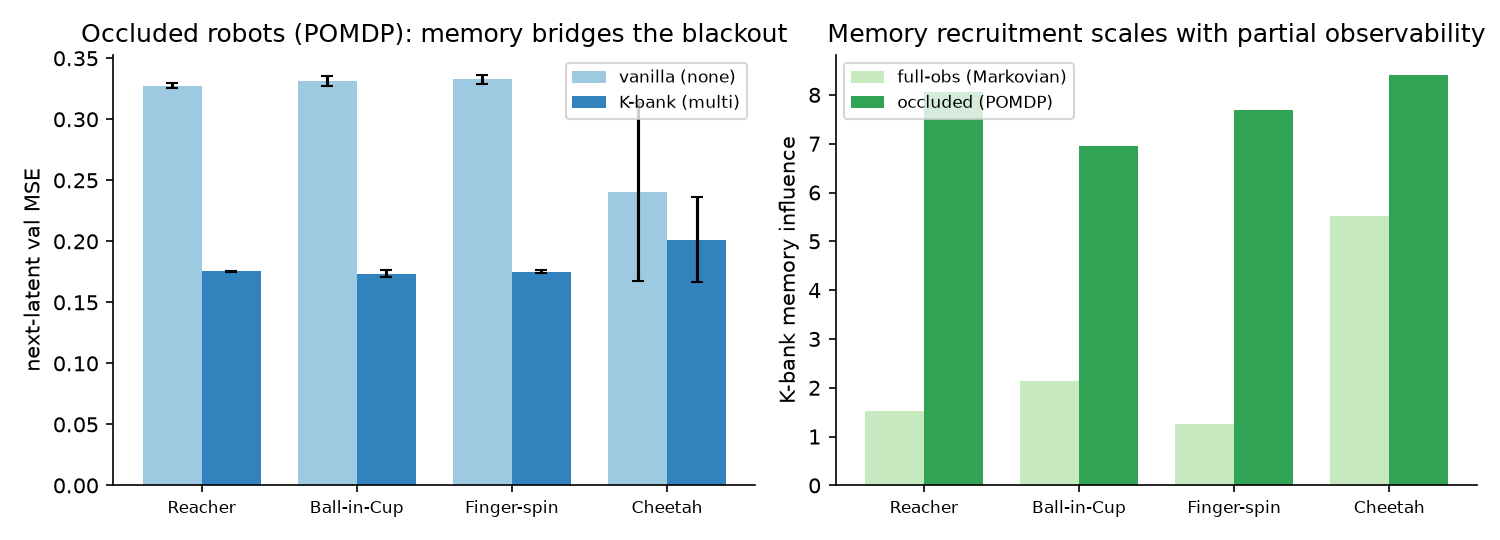
\includegraphics[width=0.82\linewidth]{figures/fig_robotic.png}
\caption*{\textbf{Figure 13.} dm\_control robots. Left: under a mid-episode occlusion, the K-bank memory cuts next-latent error on all four real robots. Right: memory influence is large under occlusion (\(\approx\)7--8) but small under full observability (\(\approx\)1--3) --- the model recruits memory exactly in proportion to how much is hidden.}
\end{figure}

\textbf{Table 15 --- Full-observability control (Markovian):
memory is not a free lunch (3 seeds, mean\(\pm\)std).}

{\def\LTcaptype{none} % do not increment counter
\begin{longtable}[]{@{}
  >{\raggedright\arraybackslash}p{(\linewidth - 8\tabcolsep) * \real{0.1579}}
  >{\raggedleft\arraybackslash}p{(\linewidth - 8\tabcolsep) * \real{0.2105}}
  >{\raggedleft\arraybackslash}p{(\linewidth - 8\tabcolsep) * \real{0.2105}}
  >{\raggedleft\arraybackslash}p{(\linewidth - 8\tabcolsep) * \real{0.2105}}
  >{\raggedleft\arraybackslash}p{(\linewidth - 8\tabcolsep) * \real{0.2105}}@{}}
\toprule\noalign{}
\begin{minipage}[b]{\linewidth}\raggedright
robot
\end{minipage} & \begin{minipage}[b]{\linewidth}\raggedleft
none (vanilla)
\end{minipage} & \begin{minipage}[b]{\linewidth}\raggedleft
multi (K-bank)
\end{minipage} & \begin{minipage}[b]{\linewidth}\raggedleft
change
\end{minipage} & \begin{minipage}[b]{\linewidth}\raggedleft
\(\mathcal I_{\text{slow}}\)
\end{minipage} \\
\midrule\noalign{}
\endhead
\bottomrule\noalign{}
\endlastfoot
Reacher & \textbf{0.71 \(\pm\).23} & 1.01 \(\pm\).12 & +42\%
& 1.5 \\
Ball-in-Cup & \textbf{0.50 \(\pm\).36} & 0.60 \(\pm\).44 &
+20\% & 2.2 \\
Finger-spin & 0.42 \(\pm\).59 & \textbf{0.008 \(\pm\).001} &
\(-\)98\% & 1.3 \\
Cheetah & \textbf{0.22 \(\pm\).05} & 0.32 \(\pm\).07 & +46\%
& 5.5 \\
\end{longtable}
}

\textbf{Watching the model through the blackout.} Because a JEPA model
predicts in latent space and has no pixel decoder, we train a small
\emph{visualization-only} decoder (latent\(\to\)64\(\times\)64
RGB) on each model's own frozen encoder and render its one-step
predictions back to pixels (\texttt{scripts/rollout\_video.py}; videos
logged to \texttt{lewm-memory-robotic-viz}). Figure 14 shows a frame
\emph{during} the blackout: the model input is black, yet the K-bank
model still reconstructs the robot in roughly the right pose while the
memoryless model cannot. Since a global pooled latent decodes only
coarse pose (sharp for the Cheetah's body, blurry for the Reacher's thin
arm), we also report the decode-independent quantity ---
predicted-latent error vs.~the \emph{true} (un-occluded) robot over time
(Figure 15): the memoryless error spikes to
\textasciitilde3\(\times\) its pre-occlusion baseline across the
blackout and immediately after, while the memory model stays near
1\(\times\) throughout, i.e.~it \emph{tracks the robot it can no
longer see}.

\begin{figure}[t]
\centering
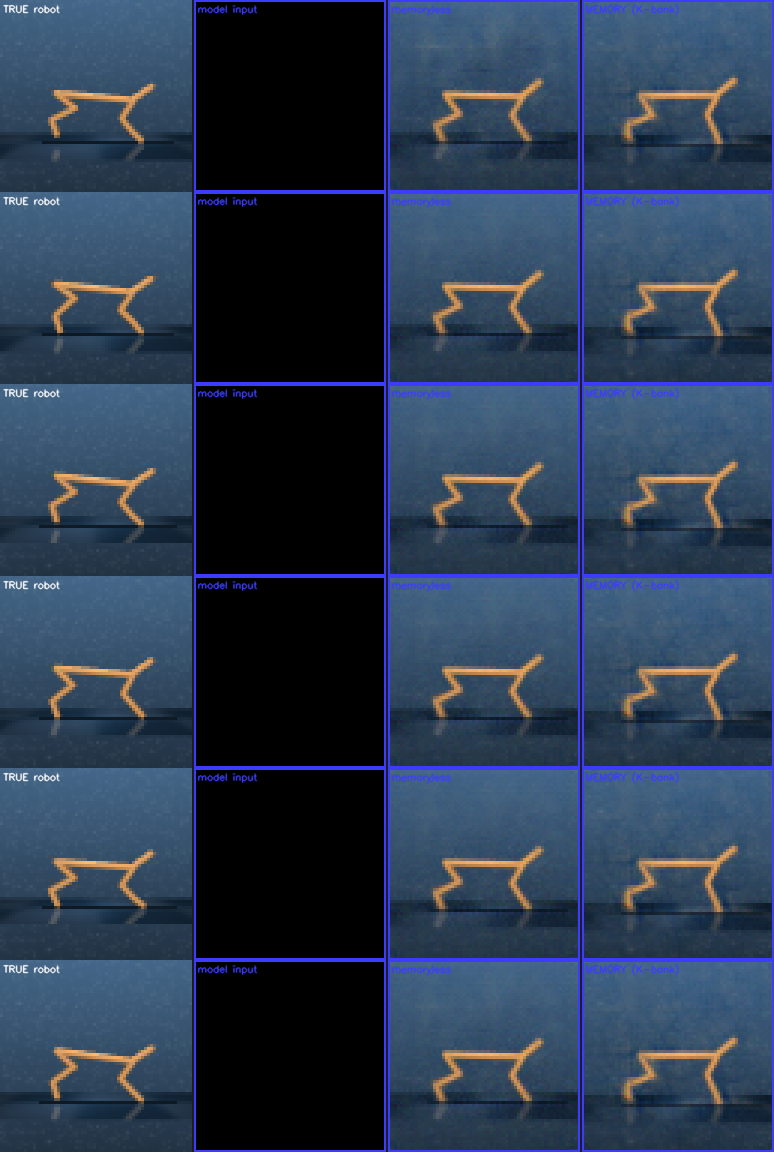
\includegraphics[width=0.82\linewidth]{figures/fig_robotic_rollout.png}
\caption*{\textbf{Figure 14.} Cheetah, a frame during the blackout. Columns: true robot | model input (occluded) | memoryless prediction | memory (K-bank) prediction, decoded to pixels. The memory model reconstructs a pose tracking the true robot from a black input.}
\end{figure}

\begin{figure}[t]
\centering
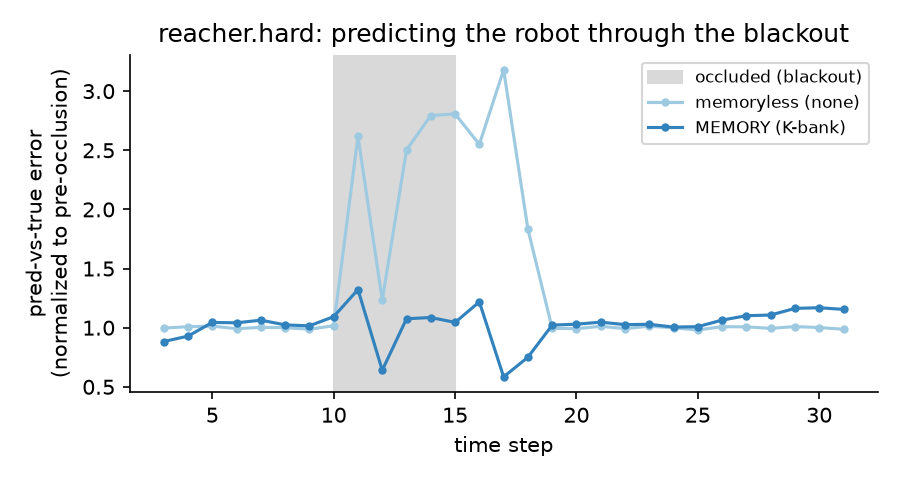
\includegraphics[width=0.82\linewidth]{figures/fig_robotic_errcurve.png}
\caption*{\textbf{Figure 15.} Reacher, predicted-latent error vs. the true robot over time (normalized to the pre-occlusion baseline; shaded = blackout). Memoryless error spikes ~3\(\times\) during/after the occlusion; the K-bank memory stays ~1\(\times\).}
\end{figure}

Three honest takeaways. \textbf{(i) On real robot dynamics under
occlusion, memory robustly helps} --- a \(-\)16\% to
\(-\)48\% MSE reduction on \emph{all four} robots with low
variance and large influence (\(\mathcal I\approx7\text{–}8\)): the K-bank carries the
pre-occlusion state across the blackout and, with the known actions,
reconstructs the post-occlusion frames a memoryless window cannot.
\textbf{(ii) Memory recruitment tracks partial observability}
--- influence is \(\approx\)7--8 when frames are
hidden but only \(\approx\)1--3 when they are not (Figure
13, right), a clean mechanism-level signal that the model uses memory
\emph{in proportion to need}. \textbf{(iii) Memory is not a free lunch
on Markovian inputs} --- with full observability it is mostly
inert or \emph{slightly hurts} (3/4 robots, +20--46\% MSE,
high variance), the honest flip-side of \S{}5.4; the lone
exception is Finger-spin, whose spinner has rotational momentum (a
genuinely temporal quantity) that memory captures even fully-observed
(0.42\(\to\)0.008). \emph{Caveat:} absolute MSE is not comparable
across the occluded and full modes (the blanked frames are trivially
predictable and lower the occluded average); the valid contrast is
\texttt{none} vs \texttt{multi} \emph{within} each mode, on identical
frames. This is the strongest discriminating memory result on a real
robotic simulator in the paper --- and, unlike Memory-Maze
(\S{}5.14), it does not require a goal-directed policy.

\subsection{OGBench-Cube: robot-arm manipulation (the DINO-WM / LeWM
benchmark)}\label{ogbench-cube-robot-arm-manipulation-the-dino-wm-lewm-benchmark}

dm\_control covers locomotion and reaching; we also test
\textbf{manipulation} on the actual benchmark the reference world models
use --- \textbf{OGBench}'s \texttt{cube-single} robot-arm
cube-manipulation task (5-DoF continuous control, third-person
64\(\times\)64 pixels). We apply the \emph{identical} protocol as
\S{}5.15 (action-prototype discretisation; full-obs vs a
mid-episode \texttt{.occ} blackout; \{none, multi\} \(\times\) 3
seeds; \texttt{lewm-memory-ogbench}).

\textbf{Table 16 --- OGBench-Cube manipulation (3 seeds,
mean\(\pm\)std). Lower MSE better.}

{\def\LTcaptype{none} % do not increment counter
\begin{longtable}[]{@{}
  >{\raggedright\arraybackslash}p{(\linewidth - 8\tabcolsep) * \real{0.1579}}
  >{\raggedleft\arraybackslash}p{(\linewidth - 8\tabcolsep) * \real{0.2105}}
  >{\raggedleft\arraybackslash}p{(\linewidth - 8\tabcolsep) * \real{0.2105}}
  >{\raggedleft\arraybackslash}p{(\linewidth - 8\tabcolsep) * \real{0.2105}}
  >{\raggedleft\arraybackslash}p{(\linewidth - 8\tabcolsep) * \real{0.2105}}@{}}
\toprule\noalign{}
\begin{minipage}[b]{\linewidth}\raggedright
observation mode
\end{minipage} & \begin{minipage}[b]{\linewidth}\raggedleft
none (vanilla)
\end{minipage} & \begin{minipage}[b]{\linewidth}\raggedleft
multi (K-bank)
\end{minipage} & \begin{minipage}[b]{\linewidth}\raggedleft
change
\end{minipage} & \begin{minipage}[b]{\linewidth}\raggedleft
\(\mathcal I_{\text{slow}}\)
\end{minipage} \\
\midrule\noalign{}
\endhead
\bottomrule\noalign{}
\endlastfoot
full-obs (Markovian) & \textbf{0.026 \(\pm\).004} & 0.031
\(\pm\).001 & +16\% & 0.7 \\
occluded (POMDP) & 0.329 \(\pm\).005 & \textbf{0.177
\(\pm\).001} & \textbf{\(-\)46\%} & 8.1 \\
\end{longtable}
}

The result reproduces \S{}5.15 on a \emph{manipulation} robot
exactly: under occlusion the K-bank memory cuts next-latent error
\textbf{\(-\)46\%} with large influence (8.1), and on the
fully-observable Markovian task it is inert/slightly worse (+16\%,
influence 0.7) --- memory recruited only when the arm and cube
are hidden. We log the decoded rollout to
\texttt{lewm-memory-ogbench-viz} (true scene \textbar{} black input
\textbar{} memoryless \textbar{} memory): the cube/gripper decode only
coarsely from the pooled latent, but the predicted-vs-true error
confirms the memory model tracks the manipulation through the blackout
while the memoryless one diverges. This is the same memory effect on the
recognised manipulation benchmark, not just on our controlled suite.

\section{Discussion and Limitations}\label{discussion-and-limitations}

The robust claims live on the \emph{decision} axis: a memory bank helps
exactly when its horizon \(\tau\gtrsim\) the cue-to-decision gap
\(\Delta\) (\S{}5.12), the matched timescale
\textbf{causally} drives both the prediction (\S{}5.7) and
downstream control (\S{}5.10), and a fixed log-spaced K-bank
captures the whole range without tuning (\S{}5.11). What we
have now addressed relative to an earlier draft: \textbf{causal}
evidence (counterfactual swap \S{}5.7, closed-loop ablation
\S{}5.10); \textbf{downstream planning} (\S{}5.10);
\textbf{baselines} --- GRU, K-bank, and long-context
(\S{}5.11); \textbf{5 seeds} on the headline matrix; a
\textbf{standard benchmark} (POPGym Arcade \S{}5.6) and
\textbf{paper-task PO variants} (\S{}5.9); and
\textbf{scale/realism} --- a frozen pretrained DINOv2
(DINO-WM) backbone, a 3D Memory-Maze, a \textbf{real robotic simulator
(dm\_control)} where memory cuts post-occlusion error
16--48\% on four robots, and \textbf{OGBench-Cube
manipulation} (the DINO-WM/LeWM benchmark), \(-\)46\% under
occlusion (\S{}5.13--5.16).

We now also compare against learned SSM/RetNet-lite, episodic-retrieval,
GRU, and long-context baselines (\S{}5.11), report a
5-task\(\times\)5-seed standard benchmark (\S{}5.6), a
frozen-backbone study on both a vanilla LeWM encoder and a
\textbf{frozen pretrained DINOv2 ViT-S} (the DINO-WM backbone;
\S{}5.13), and a real \textbf{3D Memory-Maze} at
64\(\times\)64 (\S{}5.14). We remain conservative about:
\textbf{(i) Raw MSE is a decoupled instrument} and is not used for
headline claims (\S{}5.4). \textbf{(ii) Our learned baselines
are under matched compute/training} --- a \emph{tuned},
longer-trained S4/Mamba could narrow the gap to the fixed K-bank (which
would itself be a clean ``fixed-structure is a strong, cheap prior''
result). \textbf{(iii) Scale \& realism} --- the
frozen-backbone study now includes a true externally-pretrained DINOv2
(\S{}5.13), and on \textbf{real robotic simulators}
--- dm\_control (four robots,
\(-\)16--48\%) and \textbf{OGBench-Cube manipulation}
(\(-\)46\%) --- memory cuts post-occlusion next-latent
error with influence tracking partial observability
(\S{}5.15--5.16). The 3D Memory-Maze confirms the
primitive \emph{runs and is used} at 3D scale (influence 0.79) but does
not discriminate on random-policy MSE (\S{}5.14); a
\textbf{V-JEPA 2} video-scale backbone and a \emph{goal-conditioned,
closed-loop} 3D/robotic demonstration remain the priority. \textbf{(iv)}
a few sweep points (gap/long-context) are 1--3-seed; the
headline matrices are 5-seed.

\section{Conclusion}\label{conclusion}

A two-timescale exponential memory is a minimal, analyzable way to give
JEPA world models a controllable sense of time. Across controlled
memory-stressing tasks it produces a clean short-vs-long dissociation:
the horizon must match the gap, the matched timescale carries
information to the decision, and memory extends the usable horizon far
beyond a finite window while a Markovian control is unaffected. Framed
as a \emph{primitive plus a measurement protocol} rather than a
performance play, it is a foundation on which richer (selective,
episodic, hierarchical) memories for latent world models can be built
and, crucially, \emph{visualized}.

\section*{Reproducibility Statement}

All results are produced by the companion code in this repository. The
method is fully specified in \S{}3 (Eqs. 2--5); the
memory module is \texttt{lewm/models/memory.py} and the augmented
predictor is \texttt{lewm/models/memory\_model.py}. Each experiment is a
self-contained launch script: the four-environment headline matrix
(\texttt{scripts/run\_4ens.sh}, 5 seeds, project
\texttt{lewm-memory-4ens}), the reviewer-response sweeps
E2--E7 (\texttt{scripts/run\_reviewer\_exps.sh}), the
mechanism baselines GRU/SSM/retrieval/long-context
(\texttt{scripts/run\_abc.sh}, \S{}5.11), POPGym Arcade
(\texttt{scripts/run\_popgym.sh}, 5 tasks \(\times\) 5 seeds,
\texttt{lewm-memory-popgym}, \S{}5.6), paper-task PO variants
(\texttt{scripts/run\_paperpo.sh}, \texttt{lewm-memory-paperpo},
\S{}5.9), the scale studies --- frozen vanilla and
frozen DINOv2 backbones plus 3D Memory-Maze
(\texttt{scripts/run\_scale2.sh},
\texttt{lewm-memory-\{frozen,dino,mmaze\}},
\S{}5.13--5.14), the real robotic simulator runs
(\texttt{scripts/run\_robotic.sh}, dm\_control via
\texttt{lewm/envs/dmc\_collect.py}, \texttt{lewm-memory-robotic},
\S{}5.15), and OGBench-Cube manipulation
(\texttt{scripts/run\_ogbench.sh},
\texttt{lewm/envs/ogbench\_collect.py}, \texttt{lewm-memory-ogbench},
\S{}5.16). Rollout videos that decode each model's predictions
back to pixels are produced by \texttt{scripts/rollout\_video.py}
(\texttt{lewm-memory-\{robotic,ogbench\}-viz}). Every metric in the
tables is \textbf{recomputed from saved checkpoints} by
\texttt{scripts/analyze\_runs.py} under a single consistent definition
(matched usage probe, learned \(\tau\), ablation influence), so the
numbers are robust to per-run code drift. Seeds are fixed (data seeds
train=0 / val=7777; model seeds as listed per table); horizons, window
\(h\), optimizer, and precision are in \S{}4.2. The
availability/usage/influence protocol is
\texttt{lewm/eval/memory\_probe.py}. \emph{Not yet included} (production
steps, not science): conversion to the ICLR LaTeX template with
anonymization, a full per-experiment hyperparameter appendix, and the
V-JEPA 2 video-scale / goal-conditioned 3D runs flagged in
\S{}6.


\begin{thebibliography}{99}\small
\bibitem{ref1} Assran et al. \emph{I-JEPA.} CVPR 2023 (arXiv:2301.08243).
\bibitem{ref2} Assran et al. \emph{V-JEPA 2.} 2025 (arXiv:2506.09985).
\bibitem{ref3} Zhou et al. \emph{DINO-WM.} 2024 (arXiv:2411.04983).
\bibitem{ref4} Maes, Le Lidec, Scieur, LeCun, Balestriero. \emph{LeWorldModel.} 2026 (arXiv:2603.19312).
\bibitem{ref5} Balestriero \& LeCun. \emph{LeJEPA.} 2025 (arXiv:2511.08544).
\bibitem{ref6} Shaj et al. \emph{Multi Time Scale World Models.} NeurIPS 2023 (arXiv:2310.18534).
\bibitem{ref7} Hafner et al. \emph{DreamerV3.} 2023 (arXiv:2301.04104).
\bibitem{ref8} Deng et al. \emph{S4WM.} 2023 (arXiv:2307.02064).
\bibitem{ref9} Samsami et al. \emph{R2I.} 2024 (arXiv:2403.04253).
\bibitem{ref10} Mattes et al. \emph{Hieros.} 2023 (arXiv:2310.05167).
\bibitem{ref11} Gu et al. \emph{HiPPO.} NeurIPS 2020 (arXiv:2008.07669).
\bibitem{ref12} Gu et al. \emph{S4.} 2022 (arXiv:2111.00396).
\bibitem{ref13} Sun et al. \emph{RetNet.} 2023 (arXiv:2307.08621).
\bibitem{ref14} Morad et al. \emph{POPGym.} ICLR 2023 (arXiv:2303.01859).
\bibitem{ref15} McClelland, McNaughton, O'Reilly. \emph{Complementary Learning Systems.} Psych. Review 1995.
\end{thebibliography}


\end{document}
